% lmcs, 2018.5.2, 2019.9.9, 2020.2.10



\newif\ifdraft \draftfalse
\drafttrue % put % for lipics


\long\def\Stefano#1{{{\color{red}{SB: #1}}}}
\long\def\Makoto#1{{{\color{blue}{MT: #1}}}}
\long\def\Daisuke#1{{{\color{green}{DK: #1}}}}

\ifdraft

\documentclass{article}
\usepackage{mystyle}
\A4page
%\usepackage{tikzpicture}
\usepackage{graphicx}

\else

\documentclass{lmcs}
\usepackage{hyperref}
%\usepackage{amsmath}heoremstyle{plain}\newtheorem{satz}[thm]{Satz} %\crefname{satz}{Satz}{\Succ    atze}
\usepackage{graphicx}

\fi

\usepackage{mymath,proof,latexsym}
\usepackage{xcolor}
\usepackage[pdftex,outline]{contour}


%%%%%%%%%%%%%%%%%%%%%%%%%%%%%%%%%
% AGGIUNGO TEOREMA LEMMA PROPOSIZIONE COROLLARIO PROVA % 
%%%%%%%%%%%%%%%%%%%%%%%%%%%%%%%%%

\newtheorem{theorem}{Theorem}[section]
\newtheorem{lemma}[theorem]{Lemma}
\newtheorem{proposition}[theorem]{Proposition}
\newtheorem{corollary}[theorem]{Corollary}
\newtheorem{definition}[theorem]{Definition}

\newenvironment{proof}[1][Proof]{\begin{trivlist}
\item[\hskip \labelsep {\bfseries #1}]}{\end{trivlist}}
\newenvironment{example}[1][Example]{\begin{trivlist}
\item[\hskip \labelsep {\bfseries #1}]}{\end{trivlist}}
\newenvironment{remark}[1][Remark]{\begin{trivlist}
\item[\hskip \labelsep {\bfseries #1}]}{\end{trivlist}}


\begin{document}
\sloppy 
\hbadness=10000
\vbadness=10000

% cut note 2

\def\Expand{{\rm expand}}

% cut elim

\def\RCLKIDomega{{{\bf RCLKID}^\omega}}
\def\Ren{{\rm Ren}}
\def\Terms{{\rm Terms}}
\def\IE{{\rm IE}}
\def\Cut{{\rm Cut}}
\def\Rcut{{\rm Rcut}}

% cmcs

\def\Co{{\rm co}}
\def\Axiom{{\rm Axiom}}
\def\Wk{{\rm Wk}}
\def\Cut{{\rm Cut}}
\def\BS{{\rm BS}}
\def\Bit{{\rm Bit}}
\def\LK{{\rm LK}}
\def\Head{{\rm head}}
\def\Tail{{\rm tail}}

% intuitionistic

\def\Univ{{\rm Univ}}
\def\Left{{\rm Left}}
\def\Right{{\rm Right}}
\def\Set{{\rm set}}
\def\ES{{\rm ES}}
\def\PC{{\rm PC}}
\def\Fin{{\rm Fin}}
\def\CLJIDomega{{{\bf CLJID}^\omega}}
\def\CLJIDHA{{{\bf CLJID}^\omega+{\bf HA}}}
\def\LJIDHA{{{\bf LJID}+{\bf HA}}}
\def\LJID{{\bf LJID}}
\def\OP{{\rm OP}}
\def\Div{{\rm Div}}
\def\RP{{\rm RP}}
\def\MS{{\rm MS}}
\def\ET{{\rm ET}}
\def\LiftedTree{{\rm LiftedTree}}
\def\First{{\rm first}}
\def\Er{{\rm Er}}
\def\ER{{\rm ER}}
\def\Insert{{\rm insert}}
\def\ET{{\rm ET}}
\def\SInd{{\rm SInd}}
\def\Trans{{\rm Trans}}
\def\HA{{\bf HA}}
\def\DM{{\rm DM}}
\def\Ext{{\rm ext}}
\def\KB{{\rm KB}}
\def\DT{{\rm DT}}
\def\DS{{\rm DS}}
\def\Monoseq{{\rm Monoseq}}
\def\Eq{{\rm seq}}
\def\Last{{\rm last}}

% equivalence cyclic proofs

%\def\Uor{\displaystyle \mathop {\widetilde\bigvee}}
\def\Uor{\biguplus}
\def\CLKIDomega{{{\bf CLKID}^\omega}}
\def\CLKIDPA{{{\bf CLKID}^\omega+{\bf PA}}}
\def\LKIDPA{{{\bf LKID}+{\bf PA}}}
\def\PA{{\bf PA}}

% simple equiv note

\def\LKIDN{{\bf LKIDN}}
\def\CLKIDN{{\bf CLKIDN}}

% equiv note

\def\Choose{{\rm Choose}}
\def\Asym{{\rm Asym}}
\def\Peano{{\bf Peano}}
\def\Code#1{{\lceil{#1}\rceil}}
\def\Ineq{{\rm Ineq}}
\def\MonoPath{{\rm MonoPath}}
\def\BoundedPath{{\rm BoundedPath}}
\def\InfPath{{\rm InfPath}}
\def\InfMonoPath{{\rm InfMonoPath}}
\def\HomSeq{{\rm HomSeq}}
\def\InfHomSeq{{\rm InfHomSeq}}

\def\ErdosTree{{\rm ErdosTree}}
\def\KB{{\rm KB}}
\def\MonoList{{\rm MonoList}}
%\def\Seq{{\rm Seq}}
\def\Univ{{\rm univ}}
\def\Infinite{{\rm Infinite}}
\def\S{{\bf S}}
%\def \N {{N}} %\def\N{{\bf N}} %
\def\Ind{{\rm Ind}}
\def\LKID{{\bf LKID}}
\def\PA{{\bf PA}}
\def\LKIDExt{{\bf LKIDExt}}
\def\CLKID{{\bf CLKID^\omega}}

% LICS

\def\Over#1#2{\deduce{#2}{#1}}
\def\List{{\rm List}}
\def\ListX{{\rm ListX}}
\def\ListO{{\rm ListO}}
\def\ListE{{\rm ListE}}
\def\Nl{{\rm nl}}

% CSLID

\def\SLLID{{\rm SLID}}
\def\SLID{{\rm SLID}}
\def\CSLID{{\rm CSLID}}
\def\CSLIDomega{{{\rm CSLID}\omega}}
\def\Eclass{{\rm Eclass}}
\def\Eq{{\rm Eq}}
\def\Deq{{\rm Deq}}
\def\Satom{{\rm Satom}}
\def\Cells{{\rm Cells}}
\def\Roots{{\rm Roots}}
\def\Elim{{\rm Elim}}
% \def\Case#1{{\rm Case-$#1$}}
\def\Case{{\rm Case}}
\def\Unfold{{\rm Unfold}}
\def\Pred{{\rm Pred}}
\def\Start{{\rm Start}}
\def\Unsat{{\rm Unsat}}
\def\Split{{\rm Split}}
\def\Underscore{\underline{\phantom{x}}}
\def\Rootcell{{\rm rootcell}}
\def\Rootshape{{\rm rootshape}}
\def\Jointleaf{{\rm jointleaf}}
\def\Jointleafimplicit{{\rm jointleafimplicit}}
\def\Jointnode{{\rm jointnode}}
\def\Directjoint{{\rm directjoint}}

% cyclicnote2

\def\Range{{\rm Range}}
\def\Xstart{X_{{\rm start}}}
\def\kstart{k_{{\rm start}}}
\def\Leaves{{\rm Leaves}}
\def\PureDist{{\rm PureDist}}
\def\Pure{{\rm Pure}}
\def\Identity{{\rm Identity}}
\def\Subst{{\rm Subst}}

% weak establish

\def\Connected{{\rm Connected}}
\def\Eststablished{{\rm Eststablished}}
\def\Valued{{\rm Valued}}

% monadic new

\def\SLRDbtw{{\rm SLRD}_{btw}}
\def\BTW{{{\rm BTW}}}
\def\Loc{{{\rm Loc}}}
\def\Ne{{\ne}}
\def\Nil{{{\rm nil}}}
\def\eqDef{=_{{\rm def}}}
\def\Inf#1{{\infty_{#1}}}
\def\Stores{{\rm Stores}}
\def\SVars{{{\rm SVars}}}
\def\Val{{{\rm Val}}}
\def\MSO{{{\rm MSO}}}
\def\Sep{{{\rm Sep}}}
\def\Septwo{{{\rm SLMI}}}
\def\SLMI{{{\rm SLMI}}}
\def\Sepinf{{\rm Sep}\infty}
\def\THeaps{{\rm THeaps}}
\def\Root{{\rm Root}}
\def\TG{{\rm TGraph}}

% monadic

\def\Nil{{{\rm nil}}}
\def\eqDef{=_{{\rm def}}}
\def\Inf#1{{\infty_{#1}}}
\def\Stores{{\rm Stores}}
\def\SVars{{{\rm SVars}}}
\def\Val{{{\rm Val}}}
\def\MSO{{{\rm MSO}}}
\def\Sep{{{\rm sep}}}
\def\THeaps{{\rm THeaps}}
\def\Root{{\rm Root}}
\def\TG{{\rm TGraph}}

\def\Tilde{\widetilde}
\def\Bar{\overline}
\def\Lequiv{\Longleftrightarrow}
\def\Lto{\Longrightarrow}
\def\Lfrom{\Longleftarrow}
\def\Norm{{\rm Norm}}
\def\Noshare{{\rm Noshare}}
\def\Roots{{\rm Roots}}
\def\Forest{{\rm Forest}}
\def\Var{{\rm Var}}
\def\Range{{\rm Range}}
\def\Cell{{\rm Cell}}
%\def\Tree{{\rm Tree}}
\def\Switch{{\rm Switch}}
\def\All{{\rm All}}
\def\To{\leadsto}
\def\tree{{\rm tree}}
\def\Paths{{\rm Paths}}
\def\Finite{{\rm Finite}}
\def\Const{{\rm Const}}
\def\Leaf{{\rm Leaf}}
\def\LeastElem{{\rm LeastElem}}
\def\LeastIndex{{\rm LeastIndex}}
\def\WSnS{{{\rm WSnS}}}
\def\Expand{{{\rm Expand}}}

% previous

\long\def\J#1{} % skip
\def\T#1{\hbox{\color{green}{$\clubsuit #1$}}}
\def\W#1{\hbox{\color{Orange}{$\spadesuit #1$}}}

\def\Node{{{\rm Node}}}
\def\LL{{{\rm LL}}}
\def\DSN{{{\rm DSN}}}
\def\DCL{{{\rm DCL}}}
\def\LS{{{\rm LS}}}
\def\Ls{{{\rm ls}}}

\def\FPV{{{\rm FPV}}}
\def\Lfp{{{\rm lfp}}}
\def\IsHeap{{{\rm IsHeap}}}

\def\Equiv{\quad \equiv\quad }
\def\Null{{{\rm null}}}
\def\Emp{{{\rm emp}}}
\def\If{{{\rm if\ }}}
\def\Then{{{\rm \ then\ }}}
\def\Else{{{\rm \ else\ }}}
\def\While{{{\rm while\ }}}
\def\Do{{{\rm \ do\ }}}
\def\Cons{{{\rm cons}}}
\def\Dispose{{{\rm dispose}}}
\def\Vars{{{\rm Vars}}}
\def\Locs{{{\rm Locs}}}
\def\States{{{\rm States}}}
\def\Heaps{{{\rm Heaps}}}
\def\FV{{{\rm FV}}}
\def\True{{{\rm true}}}
\def\False{{{\rm false}}}
\def\Dom{{{\rm Dom}}}
\def\Abort{{{\rm abort}}}
\def\New{{{\rm New}}}
\def\W{{{\rm W}}}
\def\Pair{{{\rm Pair}}}
\def\Lh{{{\rm Lh}}}
\def\lh{{{\rm lh}}}
\def\Elem{{{\rm Elem}}}
\def\EEval{{{\rm EEval}}}
% \def\BEval{{{\rm BEval}}} % not used 
\def\PEval{{{\rm PEval}}}
\def\HEval{{{\rm HEval}}}
\def\EVal{{{\rm Eval}}}
\def\Domain{{{\rm Domain}}}
\def\Exec{{{\rm Exec}}}
\def\Store{{{\rm Store}}}
\def\Heap{{{\rm Heap}}}
\def\Storecode{{{\rm Storecode}}}
\def\Heapcode{{{\rm Heapcode}}}
\def\Lesslh{{{\rm Lesslh}}}
\def\Addseq{{{\rm Addseq}}}
\def\Separate{{{\rm Separate}}}
\def\Result{{{\rm Result}}}
\def\Lookup{{{\rm Lookup}}}
\def\ChangeStore{{{\rm ChangeStore}}}
\def\ChangeHeap{{{\rm ChangeHeap}}}
\def\Wand{\mathbin{\hbox{\hbox{---}$*$}}}
%\def\Eval#1{[\kern -1pt[{#1}]\kern -1pt]}
\def\Eval#1{\llbracket{#1}\rrbracket}
\def\Vec{\overrightarrow}

\def\Tilde{\widetilde}
\def\Break{\hfil\break\hbox{}}

%Macro for the work on Cyclic System T with lambda
%22/03/2024
\newcommand{\ap}                { {\tt ap} }
\newcommand{\cond}            { {\tt cond} }
\newcommand{\reduces}       { \mathbin{\mapsto} }
\newcommand{\CTlambda}    { { {\tt CT} \mbox{-} \lambda} }
%\newcommand{\nameIn}       { {\tt name\mbox{-}in} }
\newcommand{\etaRule}       { {\eta\mbox{-rule}} }
\newcommand{\ins}               { {\tt ins} }
\newcommand{\struct}          { {\tt struct} }
\newcommand{\Iter}              { {\tt It} }
\newcommand{\iter}               { {\tt it} }
\newcommand{\Interval}       { {\tt In} }
\newcommand{\interval}        { {\tt in} }
\newcommand{\Succ}             { {\tt S} }
\newcommand{\nil}                { {\tt nil} }
\newcommand{\cons}             { {\tt cons} }
\newcommand{\outline}  [1]   { {\contour{black}{\textcolor{white}{#1}}}  }
\newcommand{\systemT}       { {\outline{\tt T}} }
\newcommand{\LAMBDA}       { {\outline{$\Lambda$}} }
\newcommand{\Rec}               { {\tt Rec} }
\newcommand{\rec}                { {\tt rec} }
\newcommand{\exch}             { {\tt exch} }
\newcommand{\composed}     { {\mbox{\tiny $\circ$}} }
\newcommand{\WTyped}        { {\tt WTyped} }
\newcommand{\safe}              { {\hbox{\scriptsize \tt safe}} }
\newcommand{\GlobalTraceCondition}  { {\tt GlTrCon} }
\newcommand{\Sum}              { {\tt Sum} }
\newcommand{\safeReduces} {\mathbin{\reduces_\safe}}
\newcommand{\safeReducesAst} {\mathbin{\reduces_\safe^*}}
\newcommand{\var}                { {\tt var} }
\newcommand{\Graph}            { {\tt Graph} }
\newcommand{\bfColor} [2]     {{\bf \color{#1}{#2}}}
\newcommand{\weak}             {{\tt weak}}

%colors from the web site: https://latexcolor.com/
\definecolor{amber}{rgb}{1.0, 0.75, 0.0}
\definecolor{oldgold}{rgb}{0.81, 0.71, 0.23}

\newcommand{\SubTerm}               {{\tt SubT}}
\newcommand{\Tree}                      {{\tt Tree}}
\newcommand{\N}                           {{N}}
\newcommand{\Num}                      {{\tt Num}}
\newcommand{\Nat}                        {{\outline{\tt N}}}
\newcommand{\GTC}                       {{\tt GTC}}
\newcommand{\Reg}                       {{\tt Reg}}
\newcommand{\Type}                      {{\tt Type}}
\newcommand{\conc}                      {{\star}}
\newcommand{\typingRule}            {{\tt r}}
%\newcommand{\apvar}                     {{\ap_{\mbox{\tiny var}}}}
%\newcommand{\apnotvar}               {{\ap_{\neg\mbox{\tiny var}}}}
\newcommand{\apvar}                    {{{\tt ap}_{\mbox{\tiny $v$}}}}
\newcommand{\apnotvar}               {{{\tt ap}_{\mbox{\tiny $\neg v$}}}}
\newcommand{\subseteqsim}         {{\raisebox{2pt}{$\subset$}_{\!\!\!\!\!\sim}}}
\newcommand{\supseteqsim}         {{\raisebox{2pt}{$\supset$}_{\!\!\!\!\!\sim}}}
\newcommand{\Ctxt}                       {{\tt Ctxt}}
\newcommand{\Seq}                        {{\tt Seq}}
\newcommand{\Stat}                       {{\tt Stat}}
\newcommand{\Rule}                       {{\tt Rule}}
\newcommand{\restr}                      {{\lceil}}
\newcommand{\setT}                       {{\mathcal T}}
\newcommand{\base}                      {{\tt base}}
\newcommand{\inductive}               {{\tt ind}}
\newcommand{\universe}     [1]       {{|#1|}}
\newcommand{\Label}                     {{\tt Lbl}}
\newcommand{\quotationMarks} [1]     {{\textquotedblleft#1\textquotedblright}}
\newcommand{\lexicographic} [1]   {{ <^{#1}_{\mbox{\tiny lex}}} }
\newcommand{\trunk}                     {{\tt trunk}}






\ifdraft

\title{CT-$\lambda$, a cyclic simply typed $\lambda$-calculus with fixed points}

\author{Stefano Berardi }
\date{}

\else

\title[Equivalence]
{
???
}

\author[S. Berardi]{Stefano Berardi}
\address{Universit\`{a} di Torino,
Torino, Italy}
\email{stefano@unito.it}


%% mandatory lists of keywords 
\keywords{
proof theory
inductive definitions
Brotherston-Simpson conjecture
cyclic proofs
}
\fi

\maketitle

\begin{abstract}
We explore the possibility of defining a circular syntax
directly for $\lambda$-abstraction and simple types, instead of interpreting
 $\lambda$-abstraction through combinators first, then inserting a  circular syntax afterwards.
We introduce our circular syntax as a fixed point operator defined by cases.

We prove the expected results for this circular simply typed $\lambda$-calculus, which we call $\CTlambda$: 
\emph{(i)} every closed term of type $\N$ reduces to some numeral;
\emph{(ii)}  strong normalization for all reductions sequences outside all fixed points; 
\emph{(iii)}  strong normalization for ``fair'' reductions; \emph{(iv)} Church-Rosser property;
and \emph{(i)} the equivalence between circular syntax and ordinary syntax 
for G\"{o}del system $\systemT$. 

Our motivation is that terms of $\CTlambda$ 
are much shorter than the equivalent terms written in $\systemT$.
Beside, the circular syntax of $\CTlambda$, using binders instead of combinators, 
could be more familiar for researchers working in the field of Type Theory.

\end{abstract}

\iffalse
key words: 
proof theory,
inductive definitions,
Brotherston-Simpson conjecture,
cyclic proofs,
Martin-Lof's system of inductive definitions,
infinite Ramsey theorem
Podelski-Rybalchenko termination theorem
size-change termination theorem
\fi



\section{Introduction}
We will introduce $\LAMBDA$, a set of infinite $\lambda$-terms with a circular syntax.
The types of $\LAMBDA$ are: the atomic type $\N$, 
possibly type variables $\alpha, \beta, \ldots$, and all types $A \rightarrow B$ for any types $A$, $B$. 
Type variables are only used to provide examples of terms, and they play a minor role in our paper.

The terms of $\LAMBDA$  are all possibly infinite trees representing expressions defined with 
$0$,$\Succ $,$\ap$ (application), 
variables $x^T$ (with a type superscript $T$),  $\lambda$ (the binder for defining maps), 
and $\cond$, the arithmetic conditional (i.e., the test on zero). 
If we have no term variables and no type variables, 
then the trees in $\LAMBDA$ represent partial functionals on $\N$, 
provided we add reduction rules transforming closed terms of type $\N$ in notations for natural numbers.

%19:42 19/04/2024

In this paper will consider two sets of terms: 
\begin{enumerate}
\item
the set $\CTlambda$ of well-typed terms in
a circular syntax, which are equivalent to the set of terms in G\"{o}del system $\systemT$.  
\item
The set of terms $\GTC$, satisfying a condition called global trace condition, which are possibly non-recursive
terms used to provide semantics for  $\CTlambda$ (and  $\systemT$, of course)
\end{enumerate}
We introduce more sets of terms only used 
as intermediate steps in the definition of the semantic $\GTC$ and the syntax $\CTlambda$.

\begin{enumerate}
\item
 $\WTyped \subseteq \LAMBDA$, the set of well-typed terms, is the
of set terms having a unique type
\item
$\Reg$ is the set of terms of $\LAMBDA$ which are regular trees (i.e., having finitely
many subtrees). They are possibly infinite terms which are finitely presented 
by a finite graph possibly having cycles.
\item 
$\GTC \subseteq \WTyped$ will be defined as the set of well-typed circular 
$\lambda$-terms satisfying the global trace condition (and possibly non-recursive, as we said). %and regular. 
Terms of $\GTC$ denote total functionals. 
\end{enumerate}

We will prove that $\CTlambda$ is a decidable subset of $\Reg$.
$\CTlambda$ is a new variant of the existing circular version of G\"{o}del system $\systemT$. 
Differently from all previous circular versions of $\systemT$, our system $\CTlambda$
uses binders instead of combinators. 
As we anticipated, 
 circular syntax has the advange of writing much shorter terms while preserving decidability of termination.
Besides, by introducing a circular syntax with binders, we hope to provide 
a circular syntax more familiar to researchers working in the field of Type Theory.
\\

We will prove the expected results for the circular syntax $\CTlambda$:
strong normalization for reductions not in the right-hand side of any $\cond$ and Church-Rosser. 
We will prove normalization in the limit if we use reductions which are ``fair'':
fair reductions can reduce \emph{inside} the right-hand side of some $\cond$, but they never forget entirely 
the task of reducing \emph{outside} all such subterms.

Eventually, we will prove that the closed terms $\CTlambda$ (those without free variables)
represent exactly the total computable functionals definable in G\"{o}del system $\systemT$.


%14:57 17/04/2024
%21:08 19/04/2024


\section{The set of infinite $\lambda$-terms}
We define the set $\LAMBDA$ of infinite circular terms, the subset $\WTyped$
of well-typed terms and a reduction relation for them. Infinite terms are labeled binary trees, therefore we
have to define binary trees first, and before them the lists on $\{1,2\}$ and more related notions.

\subsection{Lists and Binary Trees}

\begin{definition}[Lists on $\{1,2\}$]
\begin{enumerate}
\item
We denote with $\List(\{1,2\})$ the set of all lists of elements of $\{1,2\}$: $(),(1),(1),(1,1),(1,2),\ldots$. 
We call the elements of $\List(\{1,2\})$ just lists for short.
\item
If $i_1, \ldots, i_n \in \{1,2\}$, we write $(i_1, \ldots, i_n)$
for the list with elements $i_1, \ldots, i_n$. 
\item
We write $\nil$ for the empty list, or $()$. 
\item
If $l=(i_1, \ldots, i_n)$, $m=(j_1, \ldots, j_m)$ and $l, m \in \List(\{1,2\})$ we define
$$
l \conc m = (i_1, \ldots, i_n,\ j_1, \ldots, j_m)\in \List(\{1,2\})
$$
%If $I \subseteq \List(\{1,2\})$
%we write $l \conc I = \{l \conc m | m \in I\}$. 
\item
The prefix order $\le$ on lists
is defined by $l \le m$ if and only if $m = l \conc m'$ for some $m' \in  \List(\{1,2\})$.
\end{enumerate}
\end{definition}

Binary trees are represented by set of lists.

\begin{definition}[Binary trees]
\begin{enumerate}
\item 
A binary tree, just a tree for short, is any set $T\subseteq \List(\{1,2\})$ 
of lists including the empty list and closed by prefix: $\nil \in T$ and for all $l, m \in \List(\{1,2\})$
if $m \in T$ and $l \le m$ then $l \in T$. 
\item
$\nil$ is called the root of $T$, any $l \in T$ is called a node of
$T$ and if $l \in T$, then any $l \conc (i) \in T$ is called a child of $l$ in $T$.
\item
A node $l$ of $T$ is a leaf of $T$ if $l$ is an maximal element of $T$ w.r.t. the prefix order (i.e.,
if $l$ has no children). 
\item
If $T$ is a tree and $l \in T$ we define $T \restr l = \{m \in \List(\{1,2\}) | l \conc m \in T\}$.
$T \restr l$ is a tree and we say that $T \restr l$ is a subtree of $T$ in the node $l$,
and for each $m \in T \restr l$ we say that $l \conc m$ is the corresponding node in $T$.
\item
If $l=(i)$ we say that $T_l$ is an immediate sub-tree of $T$.
\item
A binary tree labeled on a set $L$ is any pair $\setT = (T, \phi)$ with 
$\phi:T \rightarrow L$. We call $\universe{\setT}=T$ the set of nodes of $\setT$.
For all $l \in T$ we call $\Label(\setT,l) = \phi(l)$ the label of $l$ in $\setT$.
\item
We define $\setT \restr l = (T \restr l, \phi_l)$ and $\phi_l(m) = l \conc m$. 
We call any $\setT \restr l$ a labeled subtree of $\setT$
in the node $l$, an immediate sub-tree if $l=(i)$. 
\end{enumerate}
\end{definition}

The labeling of a node $m \in \universe{( \setT \restr l )}$ 
is the same label of the corresponding node $l \conc m$ of $\universe{\setT}$.
 
Let $n = 0, 1, 2$. Assume $\setT_1, \ldots,\setT_n$ are trees labeled on $L$ and $l \in L$.
Then we define $$\setT = l(\setT_1, \ldots, \setT_n)$$ as the unique tree labeled on $L$
with the root labeled $l$ and with:
$\setT \restr (i) = \setT_i$ for all $1 \le i \le n$.


\subsection{Types, Terms and Contexts}
Now we define the types of $\LAMBDA$, then the terms and the contexts of $\LAMBDA$.

\begin{definition}[Types of $\LAMBDA$]
\mbox{}
\begin{enumerate}

\item
The types of $\LAMBDA$ are: the type $\N$ of natural numbers, an infinite list 
$\alpha,\beta,\ldots$ of type variables, and with $A,B$ also  $A \rightarrow B$.
We call them simple types, just \emph{types} for short. 

\item 
$\Type$ is the set of simples types.

\item
We suppose be given a set $\var$, consisting of all pairs $x^T=(x,T)$ 
of a variable name $x$ and a type $T \in \Type$.
\end{enumerate}
\end{definition}

Terms of $\LAMBDA$ are labeled binary trees.


\begin{definition}[Terms of $\LAMBDA$]
The terms of $\LAMBDA$ 
are all binary trees $t$ with set of labels $L=\{x^T, \lambda x^T., \ap, 0, \Succ, \cond\}$
such that:
\begin{enumerate}
\item 
a node $l$ labeled $x^T$ or $0$ is a leaf of $t$ (no children). 
\item
a node $l$ labeled $\lambda x^T.$ or $\Succ$ has a unique child $l \conc (1)$. 
\item
a node labeled $\ap$, $\cond$ has two children $l \conc (1)$, $l \conc (2)$.
\end{enumerate}
We say that $t$ is a sub-term of $u$ if $t$ is a labeled sub-tree of $u$,
an immediate subterm if it is an immediate sub-tree.
\end{definition}
 
Assume  $l \in L = \{x^T, \lambda x^T., \ap, 0, \Succ, \cond\}$.
We  use the operation $l( \setT_1 \ldots \setT_n )$ on labeled trees to define new terms in $\LAMBDA$.
If $t, u \in \LAMBDA$ then $x^T, 0, \lambda x^T.t,\ap(t,u),\Succ(t),\cond(t,u) \in \LAMBDA$ 
are terms with the root labeled $l$, and with immediate subterms among $t$, $u$. 
Conversely, each $v \in \LAMBDA$ is in one of the forms:
$x^T, 0, \lambda x^T.t$, $\ap(t,u)$, $\Succ(t)$, $\cond(t,u)$ for some $t, u \in \LAMBDA$.

Now we define the regular terms $\LAMBDA$.

%11:55 22/04/2024

\begin{definition}[Regular terms of $\LAMBDA$]
\mbox{}
\begin{enumerate}

\item
We write $\SubTerm(t)$ for the (finite or infinite) set of subterms of $t$. 
Subterms are coded by the nodes of $t$, different nodes can code the same subterm. 

\item
$\Reg$ is the set of terms $t \in \LAMBDA$ such that $\SubTerm(t)$ is finite.
We call the terms of $\Reg$ the \emph{regular terms}.

%\item
%We write $\Tree(t)$ for the tree of all chains
%$(t_1, \ldots, t_n)$ with $t_1=t$ and weakly increasing by $\sqsubset_1$: 
% for all $(i+1) \le n$ we have $t_{i+1}=t_i$ or $t_{i+1} \sqsubset_1 t_i$.

\item
As usual, we abbreviate $\ap(t,u)$ with $t(u)$.

\item
When $t = \Succ ^n(0)$ for some natural number $n \in \Nat$
we say that $t$ is a numeral. We write $\Num$ for the set of numeral in $\LAMBDA$.

\item
A variable $x^T$ is free in $t$ if there is some $l \in t$ labeled $x^T$ in $T$, 
and \emph{no $m < l$ labeled $\lambda x^T.$} in $t$. 
$\FV(t)$ is the set of free variables of $t$.
\end{enumerate}
 
\end{definition}

%We use two different names for the operation $\ap(t,u)$: 
%we call it $\ap$ when $u$ is not a variable and $\apvar$ when $u$ is a variable. 

$\Num$ is the representation inside $\LAMBDA$ of the set $\Nat$ of natural numbers.
All numerals are finite trees of $\Lambda$. 
All finite well-typed typed $\lambda$-terms 
we can define with the rules above are finite terms of $\LAMBDA$.
Regular terms can be represented by the subterm relation restricted to $\SubTerm(t)$:
this relation defines a graph with possibly cicles. Even if $\SubTerm(t)$ is finite, $t$ can be an infinite tree. 

\begin{Eg}
\label{example-regular-infinite}
An example of regular term which is an infinite tree: the term $t = \cond(0,t) \in \LAMBDA$. 
The set $\SubTerm(t)=\{t,0\}$ of subterms  of $t$ is finite, therefore $t$ is a regular term.
However, $t$ is an infinite tree (it includes itself as a subtree). 
The immediate sub-term chains of $t$ are all $(t,t,t,\ldots,t)$ and $(t,t,t,\ldots,0)$.
There is a unique infinite sub-term chain, which is $(t,t,t,\ldots)$. 
\end{Eg}

In order to define the type of an infinite term, we first 
define contexts and sequences for any term of $\LAMBDA$.
A context is a list of type assignments to variables: our variables already have a type superscript,
so in fact a type assignment $x^T:T$ is \emph{redundant} for our variables (not for our terms).
Yet, we add an assignment relation $x^T:T$ for uniformity with the notation $x:T$ 
in use in Type Theory.

%13:32 22/04/2024
%11:17 29/04/2024

\begin{definition}[Contexts of $\LAMBDA$]
\mbox{}
\begin{enumerate}

\item
A  context of $\LAMBDA$ is any finite list $\Gamma = ({x_1}^{A_1}:A_1, \ldots, x_n^{A_n}:A_n)$ 
of \emph{pairwise distinct variables}, each assigned to its type superscript $A_1, \ldots, A_n \in \Type$. 

\item
We denote the empty context with $\nil$. We write $\Ctxt$ for the set of all contexts.

\item
A sequent is the pair of a context $\Gamma$ and a type $A$, which we write as $\Gamma \vdash A$.
We write $\Seq = \Ctxt \times \Type$ for the set of all sequents.

\item 
A typing judgement is the list of a context  $\Gamma$, a term $t$ and a type $A$, 
which we write as $\Gamma \vdash t:A$.
We write $\Stat = \Ctxt \times \LAMBDA \times \Type$ for the set of all typing judgements.

\item
We write $\FV(\Gamma) = \{ {x_1}^{A_1}, \ldots, {x_n}^{A_n} \}$.
We say that $\Gamma$ is a context for $t \in \LAMBDA$ and we write $\Gamma \vdash t$ 
if $\FV(t) \subseteq \FV(\Gamma)$.

\item
If $\Gamma = ({x_1}^{A_1}:A_1, \ldots, x_n^{A_n}:A_n)$ ,
$\Gamma' = (x'_1:A'_1, \ldots, x'_n:A'_{n'})$ are context of $\LAMBDA$, then we
write 
\begin{enumerate}
\item
$\Gamma \ \subseteqsim \ \Gamma'$ \ if for all $(x^A:A)$:  \ 
$(x^A:A) \in \Gamma  \ \Rightarrow  \  (x^A:A)\in\Gamma'$
\item
$\Gamma \sim \Gamma'$  \  if for all $(x^A:A)$:  \ 
$(x^A:A) \in \Gamma  \ \Leftrightarrow  \  (x^A:A)\in\Gamma'$
\end{enumerate}


\item
If $\Gamma$ is a context of $\LAMBDA$, then $\Gamma\setminus\{x^T:T\}$ is the context obtained
by removing $x_i^{A_i}:A_i$ from $\Gamma$ for all $x_i^{A_i}=x^T$. 
If $x \not \in \FV(\Gamma)$ then $\Gamma\setminus\{x^T:T\} = \Gamma$.

\end{enumerate}
\end{definition}

We have $\Gamma \subseteqsim \Gamma'$ if and only if
if there is a (unique) map $\phi:\{1,\ldots,n\} \rightarrow \{1,\ldots,n'\}$
such that $x_{i}=x'_{\phi(i)}$ and $A_{i}=A'_{\phi(i)}$ for all $i \in \{1,\ldots,n\}$.
We have  $\Gamma \sim \Gamma'$ if and only if  $\Gamma \subseteqsim \Gamma'$
and  $\Gamma \supseteqsim \Gamma'$ if and only if $\Gamma$, $\Gamma'$ are permutation
each other if and only if the map $\phi$ above is a bijection.


%12:38 17/04/2024
%15:37 17/04/2024

%From the context for a term we can define a context for each subterm of the term.


%21:26 19/04/2024

%\begin{definition}[Inherited Contexts of $\LAMBDA$]
%
%Given any context $\Gamma$, any $t \in \Lambda$ and any subterm chain 
%$\pi = (t_1, \ldots, t_n) \in \Tree(t)$, we define a unique inherited context for $t_n$ in $\pi$.
%The inherited context is obtained by repeatedly adding $x^T:T$ to the context whenever we
%cross a term $t_i = \lambda x^T.u_i$, while simultaneously removing $x^T:T$ from the previous
%context, if it was there.
%%08:00 20/04/024
%
%\begin{enumerate}
%
%\item
%$t$ has inherited context $\Gamma$.
%
%\item
%Any binder on $x$ subtracts the variable $x$ from the context of its \emph{last} argument:
%if $t = \lambda x^T.u, \cond(f,g)$ has inherited context $\Delta$, 
%then $u$ and $g$ have context $\Delta \setminus \{x^T:T\}, x^T$, 
%while $f$ has  inherited context $\Delta$.
%
%\item
%In any other case the context of a term and of the immediate subterm are the same:
%ff $t=\Succ(u), f(a)$ have inherited context $\Delta$,
% then $u,f,a$ have  inherited context $\Delta$.
%\end{enumerate}
%We abbreviate \emph{`` inherited context from $\Gamma$''} with \emph{context}
%when $\Gamma$ is fixed.
%\end{definition}



%The scope of the binder $\lambda x^T.t$ is $t$.
%The scope of the binder $\cond(f,g)$ is $g$ ($f$ is \emph{not} in the scope of $\cond(f,g)$).

\subsection{Typing Rules}
We define typing rules for terms of $\LAMBDA$ and the subset $\WTyped$ of well-typed terms.
We consider a term well-typed if typing exists and it is unique for the term and for all its subterms.

The typing rules are the usual ones but for %the conditional binder $\cond$, and for 
the \emph{typing rule $\ap$ for an application} $t(u)$, which we split in two sub-rules, $\apvar$
and $\apnotvar$, according if $u$ is a variable or is not a variable.
%$\apvar$ corresponds to an $\eta$-expansion and it introduces a global variable name $x^T$
%for the first argument of $t$. 
%As we said, 
We need to insert this extra information $t$ in typing because it is importat for checking termination
of the computation of $t(u)$, as we will explain later.

Remark that we introduced a unique \emph{term notation}
for application: we write $\ap(t,u)$ no matter if $u$ is a variable or not, but we we split 
the typing rule for $\ap$ into two sub-cases, $\apvar$ and $\apnotvar$.

%We have a single structural rule  $\struct_f$, which can be used for:
% weakening, variable permutation and variable renaming. 
We have a a single structural rule $\weak$ for extending a context $\Gamma$ to a context 
$\Gamma' \supseteqsim \Gamma$. When $\Gamma' \sim \Gamma$ (when 
$\Gamma'$, $\Gamma$ are permutation each other), 
the rule $\weak$ can be used for variable permutation.
Variable renaming for a term $t[\vec{x}]$ can be obtained by writing 
$(\lambda \vec{x}.t[\vec{x}])(\vec{x'})$. 
Therefore we do not assume having a primitive rule for renaming. 
The lack of a renaming rule is a 
\emph{difference with the circular syntax for inductive \underline{proofs}}.

%11:56 29/04/2024

\begin{definition}[Typing rules of $\LAMBDA$]
Assume $\Gamma = {x_1}^{A_1}:A_1, \ldots, x_n^{A_n}:A_1$ is a context. 
Let $p=0,1,2$.
%$\Delta = y_1:B_1, \ldots, y_n:B_m$ are sequents of length $n$, $m$ respectively. Suppose
%$f:\{1, \ldots, n\} \rightarrow \{1, \ldots, m\}$ is any injection, compatible with types
%in $\Gamma$, $\Delta$: we assume $A_i = B_{f(i)}$ for all $1 \le i \le n$.

\begin{enumerate}
%\item
%$\struct_f$-rule.
%If $t: \Gamma \vdash T$ then $t[ y_{f(1)}/x_1, \ldots,  y_{f(p)}/x_p]:\Delta \vdash T$
\item
A rule is a list of $p+1$ typing judgements: 
$\Gamma \vdash t_1:A_1, \ldots, \Gamma \vdash t_p:A_p, \Gamma \vdash t : A$.
The first $p$ sequents are the premises of the rule (at most two in our case), 
the last sequent is the conclusion of the rule.
\item
We read the rule above: \emph{``if $\Gamma \vdash t_1:A_1, \ldots, \Gamma \vdash t_p:A_p$
then $\Gamma \vdash t : A$"}.
\end{enumerate}

We list the typing rules of $\LAMBDA$: 
the rules $\apvar$ and $\apnotvar$ are restricted.

\begin{enumerate}

\item
$\weak$-rule (Weakening).
If $\Gamma \vdash t:T$ and $\Gamma \subseteqsim \Gamma'$
then $\Gamma' \vdash t : T$

\item
$\var$-rule.
If $x^A \in \Gamma$ then $\Gamma \vdash x^A:A$.



\item
$\lambda$-rule.
If $\Gamma, x^A:A \vdash b: B$
then $ \Gamma \vdash \lambda x^A.b :A \rightarrow B$.

\item
$\apvar$-rule.
If $\Gamma \vdash f: A \rightarrow B$ then $\Gamma \vdash f(x^A) :  B$,
provided  $(x^A:A)\in  \Gamma$.

\item
$\apnotvar$-rule.
If $\Gamma \vdash f:A \rightarrow B$ and $\Gamma \vdash a:A$
then $\Gamma \vdash f(a) : B$, provided $a$ is \emph{not} a variable 

\item
$0$-rule.
$\Gamma \vdash 0: \N$

\item
$\Succ$-rule.
If $\Gamma \vdash t:\N$ then $\Gamma \vdash \Succ (t):\N$.

\item
$\cond$-rule.
If $\Gamma \vdash  f :T$ and  $\Gamma \vdash g : \N \rightarrow T$ 
then $\Gamma \vdash \cond(f,g) : \N \rightarrow T$.
\end{enumerate}
We abbreviate $\nil \vdash  t:A$ ($t:A$ in the empty context) with $\vdash t:A$. 
We write the set of rules of $\LAMBDA$ as
$$
\Rule = 
\{r \in \Seq \cup \Seq^2 \cup \Seq^3 | r \mbox{ instance of some rule of }\LAMBDA\}
$$
\end{definition}

A rule is uniquely determined from its conclusion, provided we know whether the rule is a weakening or not.
Two rules are equal if they have the same assumptions and the same conclusion.

\begin{proposition}[Rules and subterms]
\label{proposition-rules-subterms}
Assume $r, r' \in \Rule$ have conclusion $\Gamma \vdash t:A$, $\Gamma' \vdash t':A'$
respectively.
\begin{enumerate}
\item
If $r, r'$ are weakening rules and $\Gamma \vdash t:A = \Gamma' \vdash t':A'$ then $r = r'$.
\item
If $r, r'$ are non-weakening rules and $\Gamma \vdash t:A = \Gamma' \vdash' t':A'$ then $r = r'$.
\item
If $r$ is not a weakening and 
the premises of $r$ are some $\Gamma_1 \vdash t_1:A_1, \ldots, \Gamma_p \vdash t_p:A_p$,
then the list of immediate subterms of $t$ is exactly $t_1, \ldots, t_p$.
\end{enumerate}
\end{proposition}

From the typing rules we define the proofs that a term is well-typed. 
Proofs are binary trees on the set $\Rule$, each node is associated to a typing judgement which is
a consequence of the typing judgements associated to the children node under some rule $r \in \Rule$
of $\LAMBDA$.

%12:55 29/04/2024

This is the formal definition of proof.
%12:54 03/06/2024


\begin{definition}[Well-typed term of $\LAMBDA$]
Assume $\Pi=(T,\phi)$ is a binary tree labeled on $\Rule$.
Assume $\Gamma$ is a context of $t$ (i.e, $\FV(t) \subseteq \Gamma$) and $A \in \Type$ 

Then we write $\Pi: \Gamma \vdash t:A$, and we say that $\Pi$ is a proof of $\Gamma \vdash t:A$ if:

\begin{enumerate}
\item 
  $\phi(\nil) = \Gamma \vdash t:A$.
\item
  Assume that
  \begin{enumerate}
  \item
    $l \in T$ is labeled with $\phi(l) = \Delta \vdash u: B$.
  \item
    The children of $l$ in $T$ are labeled 
$
\phi(l \conc (1)) = \Delta_1 \vdash u_1: B_1, 
\ldots, 
\phi(l \conc (p)) = \Delta_p \vdash u_p: B_p
$
  \end{enumerate}
  Then for some rule $r \in \Rule$ of $\LAMBDA$ we have
  \[
  \infer[r]{
    \Delta \prove u : B
  }{
    \Delta_1  \prove u_1:B_1
    &
    \cdots
    &
    \Delta_p  \prove u_p:B_p
  }
  \]
\end{enumerate}

\end{definition}


Eventually we define the well-typed terms of $\LAMBDA$.

\begin{definition}[Well-typed term of $\LAMBDA$]
\mbox{}
\begin{enumerate}
\item
$\Gamma \vdash t:A$ is true if and only if $\Pi:\Gamma \vdash t:A$ for some $\Pi$.
\item
$t \in \LAMBDA$ is well-typed if and only if $\Pi:\Gamma \vdash t:A$ for some \emph{unique} $A$
and some context $\Gamma \supseteqsim \FV(t)$.
\item
$\WTyped$ is the set of well-typed $t \in \LAMBDA$.
\end{enumerate}
%A proof $\Pi:\Gamma \vdash  t :T$ is canonical if all $\weak$-rules
%\begin{enumerate}
%\item
% either follow some $\lambda$-rule for a term $\lambda x^T.b$, and they introduce $x^T$ in the context,
%\item
%or follow some $\cond$-rule for a term $\cond(f,g)$, and and they introduce $x^\N$ in the context,
%\end{enumerate}
\end{definition}

We provide some examples of well-typed and not well-typed terms.
%23:30 23/04/2024
Some term in $\LAMBDA$ has no type, like the application $0(0)$ of the non-function $0$. 

\begin{Eg}
We provide a term in $\LAMBDA$ having more than one type.
Let $t=u(0)$ and $u=\cond(t,u)$ 
we can prove $\vdash t:A$ for all types $A \in \Type$. 
The subterms of $t$ are $\{t, u, 0\}$ and a proof $\Pi: \emptyset \vdash t:A$ is
\[
\infer[\apnotvar]{
  \prove t : A
}{
  \infer[\cond]{
    \prove u:\N \rightarrow A
  }{
    \infer*{
      \prove t : A
    }{}
    &
    \quad
    &
    \infer*{
      \prove u : \N \rightarrow A
    }{} 
  }
  &
  \quad
  &
  \infer[0]{
    \prove 0:\N
  }{}
}
\]
Formally, the typing proof $\Pi=(T,\phi):\vdash t:A$ 
is defined by $\universe{\Pi}=\universe{t}$ and:
\begin{enumerate}
\item
$\Label(\Pi,l)=(\vdash A)$ \ \ \ \ \ \ \ for all $l \in \universe{t}$ such that  $t \restr l = t$,
\item
$\Label(\Pi,l) = (\vdash \N \rightarrow A)$  for all $l \in \universe{t}$ such that $t \restr l = u$,
\item
 $\Label(\Pi,l)=(\vdash\N)$ \ \ \ \ \ \ \  for all $l \in \universe{t}$ such that $t \restr l = 0$. 
\end{enumerate}
%09:06 24/04/2024
\end{Eg}


A term with at least two types has the leftmost branch infinite, as it is the case for $t$ above.
We will prove that if \emph{all} subterms of a term have the leftmost branch finite, then the term 
has at most one type. If the term is also regular then we can decide if the typing proof exists and 
if it exists we can compute it, in quadratic time in the size of the graph representing the term.
Well-typed terms are closed by substitution.

%10:26 20/04/2024
%13:49 29/04/2024

\subsection{Reduction Rules}
Our goal is to provide a set of well-formed term for $\LAMBDA$ and interpret them as partial functionals.
Some terms, those satisfying the global trace condition (to be introduced later) will be total functionals.
Our first step is to provide reduction rules for $\LAMBDA$.

%18:14 27/03/2024

\begin{definition}[reduction rules for $\LAMBDA$]
\mbox{}
\begin{enumerate}

\item
$\reduces_\beta$: $(\lambda x^A.b)(a) \reduces_\beta b[a/x]$

\item 
$\reduces_\cond$: $\cond(f,g)(0) \reduces_\cond f$ and
$\cond(f,g)(\Succ (t)) \reduces_\cond g(t)$.

\item
$\reduces$ is the context and transitive closure of $\reduces_\beta$ and $\reduces_\cond$

\item
$t \sim u$ if and only if there is some $v \in \LAMBDA$ such that $t \reduces v$ and $u \reduces v$.

\item
The $\cond$-depth of a node $l=(i_1, \ldots, i_n) \in t$ 
is the number of $1 \le h < n$ such that $(i_1, \ldots, i_h)$ has label $\cond$
 and $i_{h+1} = 2$
(the number of $\cond$ such that $l$ occurs in the right-hand-side of such $\cond$).

\item
We say that $t \reduces_\safe u$, or that $t$ reduces safely to $u$,  
if we only reduce on nodes of $\cond$-depth $=0$.
%We call \emph{unsafe} a reduction inside any $\cond(f,g)$.

\item
A term is safe-normal if all its redexes (if any) have $\cond$-depth $>0$.
\end{enumerate}
\end{definition}

%09:19 24/04/2024
%14:00 29/04/2024

\begin{Eg}
Let $u = \cond. (0, (\lambda z.u)(z) )$, where we omitted the type superscript
of $z$ because it is irrelevant. Then $u$ is safe-normal, because
all redexes in $u$ are of the form  $(\lambda z.u)(z)$ and are in the right-hand-side of a $\cond$. 
However, the tree form of $u$ has the following branch:
\begin{center}
  $u$, \quad
  $(\lambda z.u)(z)$, \quad
  $\lambda z.u$, \quad
  $u$, \quad $\ldots$
\end{center}
This branch is cyclic, infinite,
and it includes infinitely many $\beta$-redexes.
\end{Eg}

The reason for forbiding
reductions in the right-hand-side $\cond(f,g)$ is that through branches crossing the right-hand-side
of some $\cond$ we will-express fixed-point equations.
Reductions on fixed-point equations can easily loop, and we consider them ``unsafe". 
For this reason, we first considered the minimum possible of reductions of the form:
$\cond(f,g)(0) \reduces_\cond f$ and
$\cond(f,g)(\Succ (t)) \reduces_\cond g[t/x]$: only  those required to normalize closed
terms of type $\N$. They are the reductions \emph{applied on maximal $\cond$-expression}.
For the moment, we skip all reductions inside the second argument of $\cond$.

In a second moment, 
by adding a restriction of \emph{fairness} on reduction strategies,
we will be able to recover strong normalization for most (not all) ``unsafe" reductions.

\begin{Eg}
This is an example of safe $\cond$-reductions from a term $v(n)$ to a normal form. 
Assume $n \in \Num$ is any numeral and $v = \cond(1, v)$. There are only finitely many reductions
from $v(n)$, and they are all safe. $v(n)$ $\cond$-reduces to $v(n-1)$, 
then we loop: $v(n-1)$ $\cond$-reduces to $v(n-2)$ and so forth.
After $n$ $\cond$-reductions we get $v(0)$. With one last $\cond$-reduction we get $1$ and we stop. 
Thus, the term $v(n)$ strongly normalizes to $1$ in $(n+1)$-steps, in fact we have a unique reduction path of
length $(n+1)$ from $v(n)$ to $1$.
\end{Eg}

\section{The trace of the cyclic $\lambda$-terms}
%19:34 27/03/2024
We define a notion of trace for possibly infinite $\lambda$-terms, 
describing how an input of type $\N$ is used when computing the output.
The first step toward a trace is defining a notion of \emph{connection} between arguments
of type $\N$ in the proof that $t$ is well-typed. 
To this aim, we need the notions of \emph{list of argument
 types} and of \emph{index of atomic types} for a term.

We sketch the notion of connection through an example.
Assume 
\[
  {x_1}^{A_1}:A_1,{x_2}^{A_2}:A_2 \vdash t[x_1,x_2]:B_3 \rightarrow \N
\]
Then the list of argument types of $t$
is $A_1, A_2, B_3$. $A_1,A_2$ are arguments with names $x_1, x_2$, while $B_3$ is an unnamed
argument (it will be denoted by some bound variable in $t$). 
The index of an $\N$-argument of $t$ is any $j \in \{1,2,3\}$ such that $A_j=\N$
or $B_j=\N$ respectively: in this case all integers $1,2,3$ are indexes of some $\N$-argument,
in general we can have argument with type different from $\N$.

Remark that for an open term $ t[x_1,x_2]$ we list among the ``argument types'' also the
types $A_1, A_2$ of the free variables. We motivate this terminology:
in a sense, $t$ is an abbreviation of the closed term $t' = \lambda  
{x_1}^{A_1},{x_2}^{A_2}.t: (  A_1,A_2,B_3 \rightarrow \N )$, and the argument types of $t'$ are
$A_1, A_2, B_3$ and they include $A_1, A_2$. 

Below is the formal definition of argument types for a term.


\begin{definition}[List of argument types of a term]
Assume that $\vec{A} = A_1, \ldots, A_n$, $\vec{B}=B_{n+1}, \ldots, B_{n+m}$, 
$\Gamma = \{\vec{x}:\vec{A}\}$,
and $\Gamma \vdash t: \vec{B} \rightarrow \N$.

\begin{enumerate}
\item
The \emph{list of argument types} of $t$ is $\vec{C} = \vec{A},\vec{B}$. 

\item
$A_1, \ldots, A_n$ are the \emph{named arguments}, with names $x_1, \ldots, x_n$.

\item
$B_{n+1}, \ldots, B_{n+m}$ are the \emph{unnamed arguments}.

\item
An \emph{index of an $\N$-argument} 
of $t$ is any $j \in \{1, \ldots, n+m\}$ such that $C_j = \N$.

\end{enumerate}
\end{definition}

We now define the connection between $\N$-arguments of subterms of $t$
in a proof $\Pi: t:\Gamma \vdash A$ of  $\LAMBDA$. The connection describes
how an input  moves through the infinite unfolding of the term.
The definition of  atom connection for a syntax including the binder $\lambda$ 
is the main contribution of this paper. 
%Two $\N$-argument are in
%connection if and only if they receive the same global input: local input are ignored.
%In many cases two corresponding argument types have the same index, but if we insert or remove
%free variables or arguments the index may change.
Before providing the general definition, we discuss the notion of connection through examples. 
We draw in the same color two $\N$-argument which are in connection. 

\begin{Eg}\label{eg:0}\rm
An example of  atom connection for some instance of the $\weak$-rule.
\[
\infer[(\weak)]{
        {x_1} : \bfColor{red}{\N},{x_2} : \bfColor{blue}{\N}, x_3:\bfColor{oldgold}{\N}
		\prove t : \bfColor{orange}{\N} \rightarrow \N
}{
  {x_1} : \bfColor{red}{\N},{x_2} : \bfColor{blue}{\N} 
  \prove t : \bfColor{orange}{\N} \rightarrow \N
}
\]
\end{Eg}
Remark that the type $\N$ of the variable $x_3$, colored in \bfColor{oldgold}{old gold} and 
introduced by weakening, is in connection with no type in the rule $\weak$.

%20:13 15/04/2024
\begin{Eg}\label{eg:1}%\rm
An example of  atom connection for some instance of the $\apnotvar$-rule.
We assume that $a$ is \emph{not} a variable.
\[
\infer[(\apnotvar)]{
  x_1 : \bfColor{red}{\N},{x_2} : \bfColor{blue}{\N}
  \prove f(a) : \bfColor{orange}{\N} \rightarrow \N
}{
  x_1 : \bfColor{red}{\N},{x_2} : \bfColor{blue}{\N}
  \prove f : \bfColor{oldgold}{\N}, \bfColor{orange}{\N} \rightarrow \N
  &
  \quad
  &
  x_1 : \bfColor{red}{\N}, x_2: \bfColor{blue}{\N} \prove a : \N
}
\]
\end{Eg}
Remark that the first unnamed argument of $f$ (colored in \bfColor{oldgold}{old gold}) 
is in connection with no argument in the rule $\apnotvar$.
The reason is that in the term $f(a)$,
the first argument of $f$ receives a value from the value $a$ which is local to the term $f(a)$,
does not receive a value from outside the term.
However, the first argument of $f$ can be in connection with some argument higher in the typing proof. 
%13:21 15/04/2024

We postpone examples with the rule $\apvar$.

\begin{Eg}\label{eg:2}%\rm
An example of  atom connection for the rule $\cond$.
\[
\infer[(\cond)]{
  {x_1} : \bfColor{red}{\N},{x_2} : \bfColor{blue}{\N}
  \prove \cond(f,g) : \bfColor{oldgold}{\N} \rightarrow \N
}{
  x_1 : \bfColor{red}{\N},{x_2} : \bfColor{blue}{\N} \prove f : \N
  &
  \quad
  &
  x_1:\bfColor{red}{\N}, x_2:\bfColor{blue}{\N}, x:\bfColor{oldgold}{\N} \prove g:\N
}
\]
\end{Eg}
Remark that the first unnamed argument of $f$ (colored in \bfColor{oldgold}{old gold}) 
is in connection the type of the free variable $x$ in the second premise (the premise with $g$),
but it is in connection with no argument in the first premise (the premise with $f$).


\subsection{A formal definition of connection}
The definition of connection requires to define an injection 
$$
\ins:\N,\N \rightarrow\N
$$
We set $\ins(p,x)=x+1$ if $x \ge p+1$, and $\ins(p,x)=x$ if $x\le p$.
The role of $\ins$ is inserting one fresh index $p+1$ for a new argument type higher in the proof
connected to no argument in the conclusion.

\begin{definition}[Connection in a proof of  $\LAMBDA$]
Assume $\vec{A} = A_1, \ldots, A_n$, $\vec{B}=B_1, \ldots, B_m$, $\Gamma = \vec{x}:\vec{A}$,
and $\Gamma \vdash t:\vec{B} \rightarrow \N$.

For each $\N$-argument $k$ in $t$, for $t'=t$ or $t'$  immediate subterm of $t$ 
each $\N$-argument $k'$ in $t'$ we define the relation: ``$k',t'$ the successor of $k,t$". We require:
\begin{enumerate}
\item
if $t$ is obtained by a rule $\weak$ from $t'=t$, described by a map $\phi:\Gamma \rightarrow \Delta$,  
then $k = \phi(k')$.
\item
if $t=f(a)$ is obtained by a rule $\apnotvar$ (i.e., $a$ is not a variable) and $t'=f$ 
then $k' = \ins(n,k)$. If $t'=a$ then $k'=k$ and $k' \le n$.
\item
if $t=f(x_i^{A_i})$ is obtained by a rule $\apvar$ and $t'=f$ 
then $k' = \ins(n,k)$or $k'=n+1$ and $k=i$.
\item
if $t=\cond(f,g)$ and $t'=f$ 
then $k' = \ins(n,k)$. If $t'=g$ then $k'=k$.
\end{enumerate}
We require $k = k'$ in all other cases, 
which are: $\Succ $, $\lambda$. 
\\
No connection is defined for the rules $\var$, $0$.
\end{definition}

Below we include some examples. 
We draw in the same color two $\N$-argument which are in connection. 
In the case of the rule $\apvar$, an argument can be connected to two arguments above it.


\begin{Eg}\label{eg:3}%\rm
Atom connection for $\apvar$.
We assume that $x$ is a variable.
\[
\infer[(\apvar)]{
  x_1 : \bfColor{red}{\N},{x_2} : \bfColor{blue}{\N}, x_3  : \bfColor{oldgold}{\N}
  \prove f(x_3) : \bfColor{orange}{\N} \rightarrow \N
}{
  x_1 : \bfColor{red}{\N},{x_2} : \bfColor{blue}{\N}, x_3  : \bfColor{oldgold}{\N}
  \prove f : \bfColor{oldgold}{\N}, \bfColor{orange}{\N} \rightarrow \N
}
\]
\end{Eg}

Remark that the last variable in the conclusion of the rule
is in connection with the first unnamed argument of $f$ (colored in \bfColor{oldgold}{old gold}) 
in the premise, and with the variable with the same name in the premise: there are
two connections.

\begin{Eg}\label{eg:4}%\rm
Atom connection for  $\lambda$-rule.
We assume that $x$ is  a variable.
\[
\infer[(\ap)]{
  x_1: \bfColor{red}{\N}, x_2: \bfColor{blue}{\N}
  \prove \lambda x.b : \bfColor{oldgold}{\N} \rightarrow \N
}{
  x_1: \bfColor{red}{\N}, x_2: \bfColor{blue}{\N}, x:\bfColor{oldgold}{\N} \prove b : \N
}
\]
\end{Eg}
Remark that the first unnamed argument of $\lambda x.b$ (colored in \bfColor{oldgold}{old gold}) 
in the conclusion is in connection with the last variable type in the premise of the rule.
\\

Summing up, when
we move up in a $\apvar$-rule, the type of last free variable corresponds to the type of the first
unnamend argument.
When  we move up in a $\lambda$-rule it is the other way round. 

The connection on $\N$-arguments in a proof $\Pi:\Gamma\vdash t:A$ defines a graph $\Graph(\Pi)$ 
whose nodes are all pairs $(k,u)$, with $u$ subterm of $t$ and $k$ index of some $\N$-argument of  $u$.
$\Graph(\Pi)$ is finite when $t$ is regular.
A trace represents the movement of an input information through the infinite unfolding of a tree.
Formally, we define a trace as a (finite or infinite) path in the graph $\Graph(\Pi)$.

\begin{definition}[Trace for well-typed terms in $\LAMBDA$]
Assume $\Pi$ is any typing proof of $t \in \WTyped$.
\begin{enumerate}
\item
A path of $\Pi$ is any finite or infinite branch $\pi =(i_0, \ldots, i_n, \ldots)$ of $\Pi$.

\item
Assume $\pi =(t_0, \ldots, t_n, \ldots)$ is a path of $\Pi$, finite or infinite. 
A finite or infinite \emph{trace} $\tau$ of $\pi$ in $\Pi$ is a list 
$\tau =( (k_m,t_m), \ldots, (k_n,t_n), \ldots)$ such that for all $i=m,\ldots, n,\ldots$:
\begin{enumerate}
\item
$k_i$ is an index of some $\N$-argument of $t_i$
\item
if $i+1$ is an index of $\tau$ then $(k_{i+1},t_{i+1})$ is connected with $(k_i, t_i)$ in $\Pi$.
\end{enumerate}

\end{enumerate}
\end{definition}

The starting point of a trace could be different from the starting point of the path to which the trace belongs.

%20:50 15/04/2024
%10:35 24/04/2024
%12:28 30/04/2024

\section{The circular system $\CTlambda$}
We introduce  a condition call \emph{global trace condition} for all proofs $\Pi$ that the term $t$ is well-typed,
then the subset $\GTC$ of the set $\WTyped$ of well-typed terms of $\LAMBDA$ 
satisfying the global trace condition. $\GTC$ is a set of total recursive functionals. We use $\GTC$
as a semantics for the set $\CTlambda$ of circular $\lambda$-terms we will define.

$\CTlambda$ will be the regular terms of $\CTlambda$. 
$\CTlambda$ is a decidable set.
For the terms of $\CTlambda$ we will prove
strong normalization, church-rosser for terms of type $\N$, and the fact that every term of type
$\N$ is a numeral. 
As a consequence, all terms $\CTlambda$ will be interpreted as total functionals. 
\\

From the $\N$-argument connection we now define the global trace condition and the set of 
terms of $\GTC$  and of $\CTlambda$.



\begin{definition}[Global trace condition and terms of $\CTlambda$]
\label{definition-global-trace-condition}
\mbox{}
 \linebreak 
Assume $\tau =( (k_m,t_m), \ldots, (k_n,t_n), \ldots)$ 
is a trace of a path $\pi = (t_1, \ldots, t_n, \ldots)$ of $t \in \WTyped$. 
Assume $i=m,\ldots, n$.
\begin{enumerate}
\item
$\tau$ is progressing in $i$ if $t_i=\cond(f,g)$ for some $f$, $g$,
and $k_i$ is the index of the first \emph{unnamed} argument the $\cond$-rule, 
otherwise $\tau$ is not progressing in $i$.

\item
$t$ satisfies the global trace condition if for some typing proof $\Pi$,
of $t$, for all infinite paths $\pi$ of $t$ in $\Pi$,
there is some infinitely progressing path $\tau$ in $\pi$ and $\Pi$.
$\GTC$ is the set of $t \in \LAMBDA$ satisfying the global trace condition.

\item
$\CTlambda = \GTC \cap \Reg$: the cyclic $\lambda$-terms of 
$\CTlambda$ are all well-typed terms which are regular trees (having finitely many subtrees), 
and which satisfy the global trace condition.

\end{enumerate}
\end{definition}

The notion of global trace condition is defined through a universal quantification on proof 
$\Pi:\Gamma \vdash t:A$, and proofs $\Pi$ are possibly infinite objects and they form 
a non-countable sets.
Therefore we would expect that the global trace condition is not decidable. 
Surprisingly, global trace is decidable in polynomial space in $t$. The reason is that is some proof satisfies
the global trace condition then all proofs do, and for regular terms there is a typing proof
which is a finite graph and for which the global trace condition is decidable.

We believe that the global trace condition is decidable quite fast
for realistic $\lambda$-terms.

%18:05 03/06/2024

\section{Examples of terms of $\CTlambda$}

\subsection{The sum map}
%\Daisuke{Add sum (start)}
A first example of term of  $\CTlambda$. 
We provide an infinite regular term $\Sum$ computing the sum on $\N$.
In this example, the type superscript $\N$ of variables $x^\N$, $z^\N$ is omitted.

\begin{Eg}
\label{example-sum}
We set $\Sum = \lambda x.\cond(x,\lambda z.\Succ(\Sum(x)(z)))$.
$\Sum$ is a regular term because it has finitely many subterms: 
\begin{center}
  $\Sum$,
  \quad
  $\cond(x,\lambda z.\Succ(\Sum(x)(z)))$,
  \quad
  $x$,
  \quad
  $\lambda z.\Succ(\Sum(x)(z))$,
 \quad
  $\Succ(\Sum(x)(z))$,
  \quad
  $\Sum(x)(z)$,
  \quad
  $\Sum(x)$,
  \quad
   z
\end{center}
$\Sum$ is well-typed by the following derivation, in which we have a back edge from the 
$\bfColor{oldgold}{\dagger}$ above to the $\bfColor{oldgold}{\dagger}$ below.
\[
\infer[\lambda]{
  \vdash \Sum:\N, \bfColor{oldgold}{\N} \rightarrow \N 
   \quad (\bfColor{oldgold}{\dagger})
}{
  \infer[\cond]{
    x : \N \vdash 
    \cond(x,\lambda z.\Succ(\Sum(x)(z))): \bfColor{oldgold}{\N} \rightarrow \N
     \quad (\bfColor{oldgold}{ \spadesuit})
  }{
    \infer[\var]{
      x : \N \vdash x : \N
    }{}
    &
    \infer[\lambda]{
      x:\N \vdash \lambda z.\Succ(\Sum(x)(z)): \bfColor{oldgold}{\N} \rightarrow \N  
      %\quad (\bfColor{oldgold}{ \spadesuit})
    }{
      \infer[\Succ]{
        x:\N, z : \bfColor{oldgold}{\N} 
        \vdash \Succ(\Sum(x)(z)): \N  
        % \quad (\bfColor{oldgold}{ \spadesuit})
      }{
        \infer[\apvar]{
          x:\N, z : \bfColor{oldgold}{\N} 
          \vdash \Sum(x)(z): \N
        }{
          \infer[\apvar]{
            x:\N, z : \N
            \vdash \Sum(x): \bfColor{oldgold}{\N} \rightarrow \N
          }{
            \infer[\weak]{
              x:\N, z : \N
              \vdash \Sum: \N, \bfColor{oldgold}{\N} \rightarrow  \N
            }{
              \infer*{\vdash \Sum: \N, \bfColor{oldgold}{\N} \rightarrow \N 
                \quad (\bfColor{oldgold}{\dagger})}{}
            }
          }
        }
      }
    }
  }
}
\]
\end{Eg}

We colored in \bfColor{oldgold}{old gold} one sequence of atoms $\bfColor{oldgold}{\N}$:
this is one trace of the proof.
The colored trace is the unique infinite trace, it is cyclic and it is infinitely progressing.
We marked $\bfColor{oldgold}{ \spadesuit}$ the only progress point of the only infinite trace.
The progress point is repeated infinitely many times.


%
%\begin{tikzpicture}
%  %\draw [help lines] (-3,-1) grid (9,7);
%  \coordinate (a) at (0,0) node at (a) {A};
%  \coordinate (c) at (0,5) node at (c) {C};
%  \draw (0,0) -- (0:2cm);
%  \draw (0,0) -- (30:3cm);
%  \draw (0,5) -- +(0:2cm);
%\end{tikzpicture}

%\Daisuke{Add sum (end)}\\

%10:43 16/04/2024

\subsection{The Iterator}

\begin{Eg}
We define a term $\Iter$ of  $\CTlambda$ computing the iteration of maps on $\N$.
The term $\Iter$ is a normal term of type $(\N \rightarrow \N), \N,\N \rightarrow \N$ such that
$\Iter(f,a,n)=f^n(a)$ for all numeral $n \in \Num$. 
We have to solve the equations:

\begin{enumerate}
\item
$\Iter(f,a,0) \sim a$ 
\item
$\Iter(f,a,\Succ (t)) \sim f(\Iter(f,a,t))$
\end{enumerate}

where $f$, $a$ abbreviate $f^{\N\rightarrow\N}$ and $a^\N$.
We solve them with $\Iter = \lambda f, a.\iter$
where 
$$
\iter = \cond (a, \lambda x.f(\iter(x))):\N \rightarrow \N
$$ 
is a term in the context $\Gamma = (f:\N \rightarrow \N, a:\N)$.
\end{Eg}

\begin{proposition}
$\Iter \in \Reg \cap \WTyped \cap \GTC = \CTlambda$.
\end{proposition}

\begin{proof}
The term $\Iter$ is well-typed and regular by definition. 
We check the global trace condition. 
\\
We follow the unique infinite trace $\tau$ of the last unnamed argument $\N$ of $\Iter$ 
in the unique infinite path $\pi$ of $\Iter$. 
The trace $\tau$ moves from  $\Iter = \lambda f. \lambda a.\iter$
 to the first unnamed argument of the sub-term $\lambda a.\iter$, 
then to $a:\N$ in the context of $\iter = \cond (a, \lambda x.f(\iter(x)))$.
Then the infinite path $\pi$ and moves in this order to:
 $\lambda x.f(\iter(x))$, $f(\iter(x))$, $ \iter(x)$, $\iter$
In the meanwhile, $\tau$ progresses from $\cond$ to the second argument $\lambda x.f(\iter(x))$
of $\cond$, then moves to $x$ in the context of $f(\iter(x))$,
then to $x$ in the context $\iter(x)$, and eventually to $x$ in the context of $\iter$.
%10:30 24/03/24
In this moment the infinite path $\pi$ loops from $\iter$ to $\iter$. At each loop the trace $\tau$ 
progresses once. We conclude that $\tau$ infinitely progresses.
\end{proof}

The proof above includes a type inference from the term $\iter$ to itself.
We draw the type inference in the picture below. 
We have a back edge from the 
$\bfColor{oldgold}{\dagger}$ on the top to the $\bfColor{oldgold}{\dagger}$ in the bottom,
and we marked $\bfColor{oldgold}{ \spadesuit}$ the only progress point, which is cyclically repeated
in $\tau$.
We abbreviate $\Gamma = (f:\N \rightarrow \N, a:\N)$.
\[
%\infer[\lambda]{ %opening: \infer[\lambda]
%  \vdash \Iter:(\N \rightarrow \N), \N, \bfColor{oldgold}{\N} \rightarrow \N
% }{
%  \infer[\lambda]{ %opening: \infer[\lambda]
%  f:\N \rightarrow \N
%  \vdash \lambda a.\iter:\N, \bfColor{oldgold}{\N} \rightarrow \N
%  }
{
    \infer[\cond]{ %opening: \infer[\cond]
      \Gamma 
      \vdash \iter: \bfColor{oldgold}{\N} \rightarrow \N 
        \quad (\bfColor{oldgold}{ \spadesuit}, \bfColor{oldgold}{\dagger})
     }{ 
         \infer[\var]{
       \Gamma 
      \vdash a:\N}{}
     &
        {\ \ \ \ \ \ }
        {\infer[\lambda] %opening: \infer[\lambda]
         {
         \Gamma
          \vdash \lambda x.f(\iter(x)):\bfColor{oldgold}{\N} \rightarrow \N
         }{
         \infer[\ap]{ %opening: \infer[\ap]
           \Gamma, x:\bfColor{oldgold}{\N}
          \vdash f(\iter(x)):\N
           }{
          \infer[\var]{
       \Gamma, x:\N 
      \vdash f:\N \rightarrow \N}{}
           {\ \ \ \ \ \ \ \ \ \ \ \ }
           {\infer[\apvar] %opening: \infer[\apvar]
            {\Gamma, x:\bfColor{oldgold}{\N}
        \vdash \iter(x): \N 
             }{
          \infer[\weak]{\Gamma, x:\N
                                 \vdash \iter: \bfColor{oldgold}{\N} \rightarrow \N}
                                {\infer*{\Gamma
                                 \vdash \iter: \bfColor{oldgold}{\N} \rightarrow \N
                                  \ \ \ (\bfColor{oldgold}{ \dagger})}{}
             }
           }
          }
        }%closing: \infer[\apvar]
      }%closing: \infer[\ap]
    }%closing: \infer[\lambda]
   }%closing: \infer[\cond]
 }%closing: \infer[\lambda]
%}%closing: \infer[\lambda]
\]




\subsection{The Interval Map}
A third example. We simulate lists with two variables $\nil:\alpha$ and 
$\cons:\N,\alpha \rightarrow \alpha$. We recursively define a notation for lists by $[]=\nil$,
$a @ l=\cons(a,l)$ and $[a,\vec{a}] = a @ [\vec{a}]$. We add no elimination rules for lists, though,
only the variables $\nil$ and $\cons$. Elimination rules are not required in our example.

\begin{Eg}
We will define a term $\Interval$ with one argument $f:\N \rightarrow \N$ and three argument
$a,x,y:\N$ (we skip all type superscripts), such that 
\[
\Interval(f,a,n,m) \  \sim \ [f^n(a), f^{n+1}(a), \ldots, f^{n+m}(a)] \  : \ \alpha
\]
for all numeral $n,m \in \Num$. 
We have to solve the recursive equations 
\begin{center}
  $\Interval(f,a,n,0) \sim [f^n(a)]$
  \quad
  and
  \quad
  $\Interval(f,a,n,\Succ (m))  \sim f^n(a) @ \Interval(f,a,\Succ(n),m)$.
\end{center}
Assume $\iter = \cond (a, \lambda x.f(\iter(x))):\N \rightarrow \N$ is the term
in the context $(f:\N\rightarrow\N, a:\N)$ defined 
in the previous sub-section: in particular, $\iter(n) \sim f^n(a)$ for all $n \in \Num$.
We solve the recursive equation for $\Interval$ with $\Interval = \lambda f,a.\interval$,
where 
\[
\interval:\N,\N \rightarrow \alpha
\]
is a term in the context $(f:\N\rightarrow\N, a:\N)$ defined by 
\[
\interval 
\ \ \ = \ \ \ 
\lambda x.\cond (\base,  \lambda y.\inductive),
\]
where the base case and the inductive case are
\[
\base 
\ \ \ =\ \ \  
[\iter(x)]
\ \ \ =\ \ \ 
\cons(\iter(x),\nil)
\]
\[
\inductive 
\ \ \ = \ \ \ 
\iter(x) @ \interval(\Succ(x))(y)
\ \ \ = \ \ \  
\cons(\ \iter(x), \ \interval(\Succ(x))(y) \ )
\]
\end{Eg}

\begin{proposition}
$\Interval \in \Reg \cap \WTyped \cap \GTC = \CTlambda$.
\end{proposition}

\begin{proof}
The term $\Interval$ is well-typed and regular by definition. We check the global trace condition.
Any infinite path $\pi$ either moves to $\iter$, for which we already checked the global trace condition,
or cyclically moves from $\interval$ to $\interval$.
We follow the unique infinite 
trace $\tau$ of the last unnamed argument $\N$ of $\Interval$ inside this infinite path.
The trace $\tau$ moves to the last unnamed argument $\N$ of  
$\interval:\N,\N \rightarrow \N$, then to the last unnamed argument of
$\cond (\ [\iter(x)],  \  \lambda y.\iter(x) @ (\lambda x.\interval)(\Succ(x))(y) \ )$.
In this step $\tau$ progresses, and moves to 
the first unnamed argument of $\lambda y.\iter(x) @ (\lambda x.\interval)(\Succ(x))(y) \ )$,
then to $y:\N$ in the context of $\iter(x) @ (\lambda x.\interval)(\Succ(x))(y) \ )$.
After one $\apvar$ rule, the trace $\tau$ reaches the unique unnamed argument of 
$(\lambda x.\interval)(\Succ(x))$, then the last unnamed argument $\tau$ of $\interval$. 
From $\interval$ the trace $\tau$ loops. Each time $\tau$ moves from $\interval$ to $\interval$
then $\tau$ progresses once. We conclude that $\tau$ infinitely progresses.
\end{proof}
%14:27 24/04/2024

The proof above includes a type inference from the term $\interval$ to itself.
We draw the type inference in the figure \ref{figure-term-interval}. 
In this figure, we include a back edge from the 
$\bfColor{oldgold}{\dagger}$ on the top to the $\bfColor{oldgold}{\dagger}$ in the bottom,
and we marked $\bfColor{oldgold}{ \spadesuit}$ the only progress point, which is cyclically repeated
in $\tau$.
We abbreviate 
$\Sigma = (\nil:\alpha, \cons:\N,\alpha \rightarrow \N)$
and
$\Gamma = \Sigma,(f:\N \rightarrow \N, a:\N)$.

%PROOF SNAPSHOT
\begin{figure}
\label{figure-term-interval}

%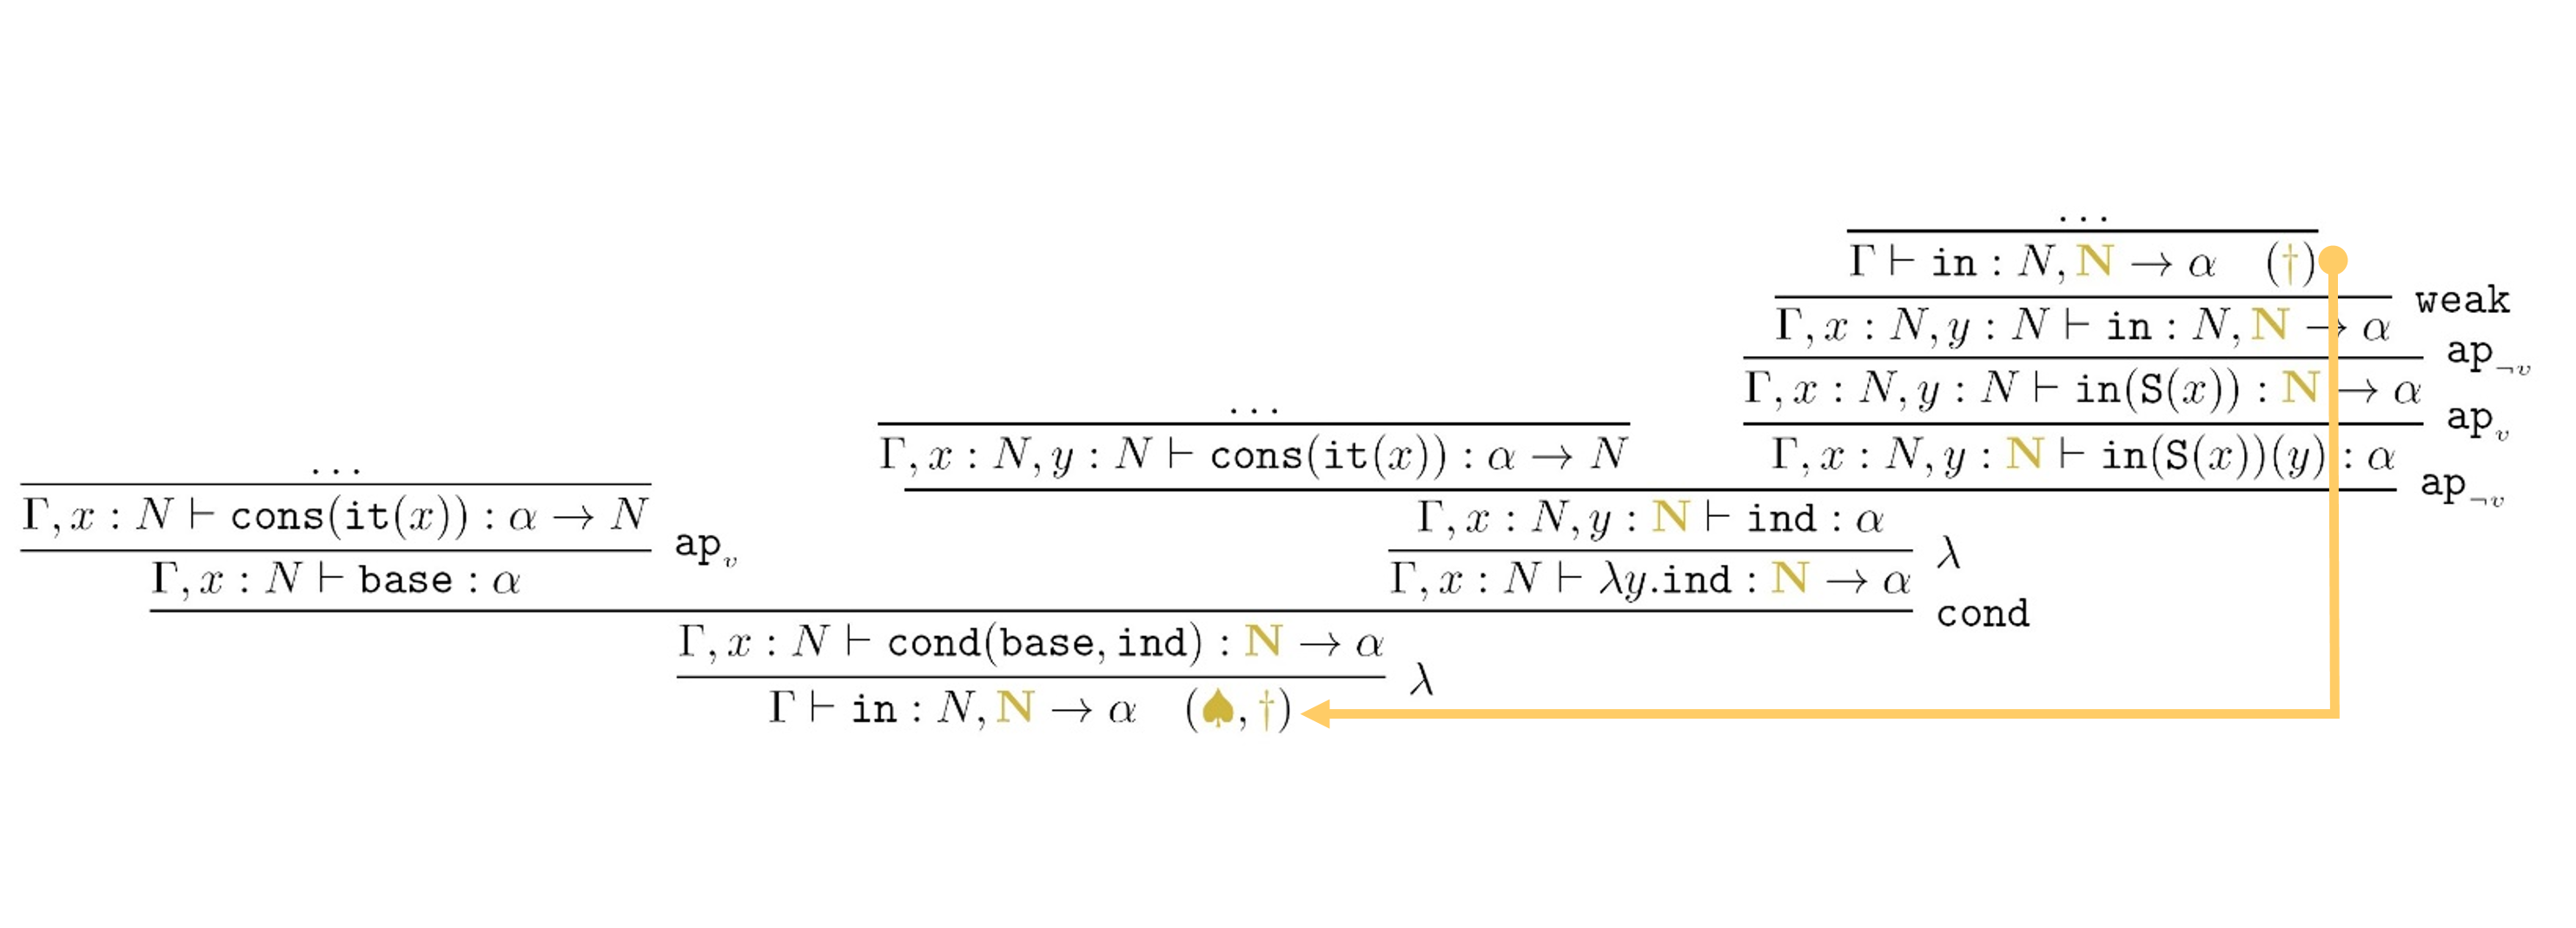
\includegraphics[scale=0.6]{type-inference-term-interval.PNG}

\begin{center}
%% LATEX SOURCE CODE THEN A SNAPSHOT 
%% THEN THE SNAPSHOT HAS BEEN MODIFIED IN WORD 
%% THEN A LAST SNAPSHOT
  
\[
%\infer[\lambda]
% {\Sigma\vdash \Interval:(\N \rightarrow \N),\N,\N,\bfColor{oldgold}{\N}\rightarrow\alpha}
% {\infer[\lambda]
%   {\Sigma,f:\N\rightarrow\N \vdash \lambda a.\interval:\N,\N,\bfColor{oldgold}{\N}   
%      \rightarrow\alpha}
   {\infer[\lambda]  
     {\Gamma \vdash \interval:\N,\bfColor{oldgold}{\N}\rightarrow\alpha 
       \ \ \ (\bfColor{oldgold}{\dagger}) }
       {\infer[\cond]{\Gamma, x:\N 
	\vdash 
	\cond (\base,  \inductive )
	:\bfColor{oldgold}{\N}\rightarrow\alpha \ \ \ (\bfColor{oldgold}{ \spadesuit}) } 
       {\infer[\apvar]{\Gamma, x:\N 
	           \vdash 
	           \base:\alpha}
             {\infer[]{\Gamma, x:\N 
	           \vdash 
	           \cons(\iter(x)):\alpha \rightarrow\N}{\ldots}}
            {\ \ \ \ \ \ }  &
          \infer[\lambda]{\Gamma, x:\N 
	           \vdash 
	           \lambda y.\inductive : \bfColor{oldgold}{\N}\rightarrow\alpha}
             {\infer[\apnotvar]{\Gamma, x:\N, y:\bfColor{oldgold}{\N} \vdash
               \inductive : \alpha}
            {\infer[]
                     {\Gamma, x:\N, y:\N 
                          \vdash \cons(\iter(x)):\alpha\rightarrow\N}{\ldots}
               {\ \ \ \ \ \ }
                     {\infer[\apvar]{\Gamma, x:\N, y:\bfColor{oldgold}{\N} 
                          \vdash \interval(\Succ(x))(y):\alpha}
                         {\infer[\apnotvar]{\Gamma, x:\N, y:\N 
                          \vdash \interval(\Succ(x)):\bfColor{oldgold}{\N} \rightarrow\alpha}
                              {\infer[\weak]{\Gamma, x:\N, y:\N 
                          \vdash \interval:\N,\bfColor{oldgold}{\N} \rightarrow\alpha}
                                {\infer[]{\Gamma 
                          \vdash \interval:\N,\bfColor{oldgold}{\N} \rightarrow\alpha
                           \ \ \ (\bfColor{oldgold}{\dagger})}
              {\ldots}}}}}
             }
           }
         }
       }  
    }
%   }
\]

\mbox{Figure \ref{figure-term-interval}}
\end{center}

\end{figure}

If we carefully examine the term $\Interval$, we can guess several results of this paper.
We have infinitely many nested $\beta$-reduction $(\lambda x. \ldots)(\Succ (x))$.
We can remove all of them in a single step. Inside the $\beta$-redex number $k$ we obtain a sub-term
$\iter[\Succ (x)/x]\ldots[\Succ (x)/x]$ (substitution repeated $k$ times).
The result is $\iter[\Succ ^k(x)/x] $.
The nested substitution produce infinitely many pairwise different sub-terms 
$\iter(\Succ ^k(x))$ for all $k \in \N$.
We need infinitely many steps to normalize all $\iter(\Succ ^k(x))$ to $f^k(I)$, 
even if we allow to reduce all $\beta,\cond$-redexes at the same time.
Also the normal form is not regular: it contains all terms $f^k(\iter(x))$ for $k \in \N$, hence
infinitely many pairwise different terms. 
%These infinite sub-terms are of a particulary simple form, though. 
%They are obtained by the repeating $k$ times the assignment $z:=f(z)$, then applying $z:=I$ once
%to the result.

In conclusion, 
$\Interval$ is some term of $\CTlambda$ which can be safely normalized, but which 
cannot be fully normalized in finite time, not even if we allow
infinite parallel reductions without any "safety" restriction. 
The normal form is produced \emph{only in the limit}
and it is \emph{not regular}. If we allow to reduce infinitely many nested existing
$\beta$-redexes in one step, also
the intermediate steps of the infinite reduction of $\Interval$ are not regular.

%16:32 30/04/2024

%22:30 03/06/2024

\section{Subject reduction for terms of $\WTyped$ of type $\N$}
\label{section-subject-reduction}
%\Daisuke{SR start}
\ldots\ldots\ldots\ldots\ldots\ldots\ldots\ldots\ldots\ldots
\\
\bfColor{red}{(Here we should fill this part - Daisuke)}
\ldots\ldots\ldots\ldots\ldots\ldots\ldots\ldots\ldots\ldots
%\Daisuke{SR end}


\section{Church-Rosser for Infinite Lambda Terms}
\label{section-church-rosser}
%15:12 16/04/2024
\ldots\ldots\ldots\ldots\ldots\ldots\ldots\ldots\ldots\ldots
\\
\bfColor{red}{(Here we should fill this part - Stefano)}
\ldots\ldots\ldots\ldots\ldots\ldots\ldots\ldots\ldots\ldots
%15:46 24/04/2024


\section{Finiteness of Safe Reductions for $\GTC$}
\label{section-finiteness-safe-reductions}
In this section we use Church-Rosser for $\LAMBDA$.
We prove that every infinite reduction sequence of $\GTC$ includes
only finitely many "safe" reduction steps. This implies that sequences of "safe" reduction steps of $\GTC$
are finite, that is, strong normalization for "safe" reduction steps.
\\

In the following, we explicitly write $t[x_1,\ldots,x_n]$,
when each free variable in  a term $t$ is some $x_i$, 
and, under this notation, we also write $t[a_1,\ldots,a_n]$ instead of $t[a_1/x_1,\ldots,a_n/x_n]$. 

We define total well-typed terms by induction on the type, as in Tait's normalization proof.

\begin{definition}[Total well-typed terms of $\LAMBDA$]
\label{definition-total-term}
Let $u \in \LAMBDA$.
$u$ is \emph{finite for safe reduction} if and only if all infinite reduction sequences from $t$ 
include only finitely many "safe" reduction steps.  
Let $t \in \WTyped$, $t : T$.

 
We define \quotationMarks{$t$ is total of type $T$} by induction on $T$

\begin{enumerate}
\item
Let $T$ be any atomic type: $T = \N$ or $=\alpha$ for some type variable $\alpha$.
Then $t$ is total of type $T$ if and only if $t$ is finite for safe reductions.

\item
Let $T$ be any arrow type $A \rightarrow B$.
Then $f$ is total of type $T$ if and only if for all total $a$ of type $A$ we have $f(a)$ total of type $B$.
\end{enumerate}

A \emph{total assignment} $[\vec{x}/\vec{v}]$ 
is any assignment of total terms to variables of the same type.

A term $t$ is \emph{total by substitution} if and only if:
$t[\vec{x}/\vec{v}]$ is total for all total assignments $[\vec{x}/\vec{v}]$
\end{definition}

By definition, any total term is well-typed, in particular it has exactly one type.

We define the safe trunk of a term as the part of the term which we can normalize with safe reductions only,
and  the $\Succ$-length of a term $t \in \LAMBDA$ the number of $\Succ$ in front of the safe trunk.
Here is the formal definition.

\begin{definition}[$\Succ$-length]
Assume $t \in \LAMBDA$
\begin{enumerate}
\item
The safe trunk of $t$ is any expression $u[\cond(f_1,\cdot), \ldots, \cond(f_n,\cdot)]$
such that  for some $g_1, \ldots, g_n$ we have $v = u[\cond(f_1,g_1), \ldots, \cond(f_n,g_n)]$
\emph{safe normal} and $t \reduces v$.
\item
The $\Succ$-length of $t$ is
the number of $\Succ$ in front of any safe-normal form of $t$, if any exists. 
\end{enumerate}
\end{definition}


\begin{Eg}
The $\Succ$-length is a kind a value we can assign to \emph{all} terms of $\LAMBDA$.  
We compute the $\Succ$-length for some normal terms of $\LAMBDA$.
$0$ has $\Succ$-length $0$, $\Succ(x)$ has $\Succ$-length $1$, 
$\Succ(\Succ(\cond(f,g)(x))$ has $\Succ$-length $2$, while $t = \Succ(t)$ has infinite $\Succ$-length.
\end{Eg}

The $\Succ$-length exists for total terms.
From the Church-Rosser property for $\LAMBDA$ (\S \ref{section-church-rosser})
we deduce that the $\Succ$-length is unique when it exists.

\begin{lemma}[$\Succ$-length of terms  finite for safe reductions]
\label{lemma-succ-length}
Assume $t \in \LAMBDA$.

\begin{enumerate}
\item 
\label{lemma-succ-length-01}
The safe-trunk and $\Succ$-length exist and they are unique. 

\item
\label{lemma-succ-length-02}
If $t \reduces \Succ(u)$, then the $\Succ$-length of $u$ is $1$ unit 
smaller than the $\Succ$-length of $t$.

\end{enumerate}
\end{lemma}



\begin{proof}
Assume $t \in \LAMBDA$.

\begin{enumerate}
\item
%\label{lemma-succ-length-01}
Assume that $u[\cond(f_1,\cdot), \ldots, \cond(f_n,\cdot)]$ and
$u'[\cond(f'_1,\cdot), \ldots, \cond(f'_{n'},\cdot)]$ are safe-trunks for $t$, in order to prove
that $u=u'$ and $n=n'$. 

Then for some $g_1, \ldots,g_n$ and some $g'_1, \ldots,g'_n$ we have that 
$v = u[\cond(f_1,g_1), \ldots, \cond(f_n,g_n)]$ and 
$v' = u'[\cond(f'_1,g'_1), \ldots, \cond(f'_n,g'_{n'})]$ 
are safe-normal forms of $t$ and all $\cond$-expressions shown are maximal. 
The decomposition of each safe-normal form $v$ is therefore unique:
if $v = u"[\cond(f"_1,g"_1), \ldots, \cond(f"_n,g"_{n"})]$ then $u=u"$ and $n=n"$.
Each reduction from any of the safe-trunks takes place in some $g_1, \ldots,g'_{n'}$. 

By Church-Rosser  (\S \ref{section-church-rosser}) we deduce that $v$ and $v'$ are confluent, therefore
for some $v"$ we have $v, v' \reduces v"$. Since the reductions on $v, v'$ take place in some $g_1, \ldots,g'_{n'}$, we deduce that $v" = u[\cond(f_1,g"_1), \ldots, \cond(f_n,g"_n)]$
and $v" = u[\cond(f_1,g'"_1), \ldots, \cond(f_n,g'"_{n'})]$ for some $g"_1, \ldots,g'"_{n'}$.
From the unicity of the decomposition of $v"$
with maximal $\cond$-subterms we conclude that $u=u'$ and $n=n'$. 
\\

From unicity of the safe-trunk we deduce that the $\Succ$-length is unique.

\item
%\label{lemma-succ-length-02}
\emph{Assume that $t \reduces \Succ(u)$, in order to prove that 
the $\Succ$-length of $u$ is $1$ unit smaller than the $\Succ$-length of $t$}.
By the point \ref{lemma-succ-length-01} above, 
$u$ has $\Succ$-length some $k \in \N$. Then $u \reduces \Succ^k(v)$
for some $v$ not successor, 
therefore $t \reduces \Succ^{k+1}(v)$ and the $\Succ$-lenght of $t$ is $\ge k+1$.

\end{enumerate}
\end{proof}


We will assign total terms to  the sub-terms of $t$
in an infinite path of a proof $\Pi : \Gamma \vdash t: A$ in a way compatible with traces. 


\begin{definition}[Trace-compatible Assignment]
\label{definition-trace-compatible}
Assume $\pi  = (\Gamma_1 \vdash t_1:A_1, \ldots, \Gamma_n \vdash t_n:A_n, \ldots)$ 
is any finite or infinite branch of $\Pi$
and $\vec{v} = (\vec{v_1}, \ldots, \vec{v_n}, \ldots)$ 
is any sequence of total assignments, one for each $t_i$. 
$\vec{v}$ is \emph{trace-compatible} in an index $i$ of $\pi$  
if and only if it satisfies the following condition:

  for all $j$  index of an $\N$-argument of $t_i$ with $v_j$ of $\Succ$-length $a$, 
  all $k$ index of an $\N$-argument of $t_{i+1}$ with $v_k$ of $\Succ$-length $b$, 
  if $j$ is connected to $k$ then:
 \begin{enumerate}
 \item
 if $j$ progresses to $k$ then $a=b+1$
 \item
 if $j$ does not progress to $k$ then $a=b$.
 \end{enumerate}
$\vec{v}$ is \emph{trace-compatible} if it is trace-compatible in all $i$.
\end{definition}

If an infinite path has a trace-compatible assignment, 
then all traces of the path progress only finitely many times.

\begin{proposition}[Trace assignment]
\label{prop:trace_assign-finiteness}
Assume $\Pi:\Gamma \vdash t:A$ and there is some infinite path $\pi$ of $\Pi$ and
some a trace-compatible assignment  $\rho$ to $\pi$. Assume $n \in \Nat$.
\begin{enumerate}
\item
\label{prop:trace_assign-finiteness1}
If an $\N$-argument $j$ of some $t_i \in \pi$ has $\Succ$-length $n$ in $\rho$, then a trace
from $j$ progresses at most $n$ times.
\item
\label{prop:trace_assign-finiteness2}
$t \not \in \GTC$.
\end{enumerate}
\end{proposition}

\begin{proof}
\begin{enumerate}
\item
%\label{prop:trace_assign-finiteness1}
By definition of trace-compatible assignment, whenever the trace progresses, 
the $\Succ$-length $n$ associated to the progressing argument decreases by $1$.
Whenever the trace does not progress, the numeral $n$ remains the same.
Thus, a trace from $j$ progresses at most $n$ times, as we wished to show.
\item
%\label{prop:trace_assign-finiteness2}
By point \ref{prop:trace_assign-finiteness1} above, 
no trace from any argument in any term of the branch $\pi$ of $\Tree(t)$ progresses infinitely many times.
We assumed that there is an infinite path $\pi$ in $\Pi$.
By definition of $\GTC$, we conclude that $t \not \in \GTC$. 
\end{enumerate}
\end{proof}


We now continue with our Tait's style proof of Strong Normalization.
We check that total terms are closed by reductions, by application and by variables.
Any total term is finite for safe reductions.




\begin{lemma}\label{lem:total_value-finiteness}
Assume $t,u,f,a \in \WTyped$ and $A,B,T$ are types.

  \begin{enumerate}
  \item
\label{lem:total_value-finiteness1}
    Let $t:A$ and $t \reduces u$.
    If $t$ is total, then $u$ is total.

  \item
\label{lem:total_value-finiteness2}
    If $f:A \rightarrow B$ and $a:A$ are total terms, then $f(a)$ is total.

  \item
\label{lem:total_value-finiteness2bis}
    $x^T:T$ is total.

 \item
\label{lem:total_value-finiteness2ter}
  If $t$ is total then $t$ is finite for safe reductions.

  \item
\label{lem:total_value-finiteness3}
    Let $T$ be any atomic type, and $t[\vec{x}]:\vec{A}\rightarrow T$ be a term
    whose all free variables are $\vec{x}:\vec{B}$.

    If for all total $\vec{u}:\vec{B}$, $\vec{a}:\vec{A}$ the term 
    $t[\vec{u}]\vec{a}:\N$ is \emph{finite for safe reductions}, then
    the term $t[\vec{x}]$ is \emph{total by substitution}.
  \end{enumerate}

\end{lemma}




\begin{proof}
\begin{enumerate}

\item
%\label{lem:total_value-finiteness1}
  We show \emph{point \ref{lem:total_value-finiteness1}}  by induction on $A$. 
We assume that $t:A$ and $t \reduces u$.
    and $t$ is total, in order to prove that $u$ is total.By the subject reduction property, $u$ has type $A$.
\begin{enumerate}
\item
  We show the \emph{base case}, namely when $A =\N,\alpha$ is an atomic type.
  By the assumption, $u$ is total.
  By definition of $t$ total for $T$ atomic, all infinite 
  reductions from $t$ only include finitely many safe reductions.
  All infinite reductions from $u$ can be extended to some infinite reduction from $t$, and therefore they
  only include finitely many safe reductions.
\item
  We show the \emph{induction case}, namely when $A = (A_1\rightarrow A_2)$.
  Take any arbitrary total term $a:A_1$ in order to prove that $u(a):A_2$ is total. 
  Then we have $t(a) \reduces u(a)$ and 
  $t(a):A_2$ is total by the assumption that $t$ is total.
  Hence $u(a)$ is total by $t(a) \reduces u(a)$ and the induction hypothesis on $A_2$. 
  We conclude that $u:A_1\rightarrow A_2$ is total. 
\end{enumerate}

  \item
%\label{lem:total_value-finiteness2}
If $f:A \rightarrow B$, $a:A$ are total  terms, then $f(a)$  is total by definition of total.

\item
%\label{lem:total_value-finiteness3}
We prove that $x^T:T$ is total. 
We prove that for all total $\vec{a}:\vec{A}$, if $T = \vec{A} \rightarrow U$ then $x(\vec{a}):U$
is total. The thesis follows if we take $\vec{a} = \nil$. We argue by induction on $U$. 

\begin{enumerate}
\item
Assume $U$ is atomic. Then every reduction on $x(\vec{a}):U$
takes place in $\vec{a}$. By definition of total
for an atomic type we have to prove that in all infinite reduction sequences from $x(\vec{a}):U$ 
there are only finitely many safe reduction. All reductions on $x(\vec{a})$ take place on $\vec{a}$,
and since each $a_i$ in $\vec{a}$ is total only finitely many safe reductions are possible, as we wished.
\item
Assume $U = (A_1 \ldots A_2)$. By definition of total
for an arrow type we have to prove that for all total $a$ we have  $x(\vec{a},a):A_2$ total.
This follows by induction hypothesis on $A_2$.
\end{enumerate}

\item
%\label{lem:total_value-finiteness4}
\emph{We assume that  $t:U$ is total in order to prove that $t$ is finite for safe reductions}.
We argue by induction on $U$.
\begin{enumerate}
\item
If $U$ is atomic then the thesis is true by definition of total.
\item
Suppose $U = (A_1 \rightarrow A_2)$. By point \ref{lem:total_value-finiteness3} above,
$x^{A_1}:A_1$ is total, therefore $t(x):A_2$ is total and by induction hypothesis on $A_2$
any infinite reduction sequence from $t(x)$ only includes finitely many safe reductions. 
Any infinite reduction sequence 
$\sigma: t = t_0 \reduces_1 t_1 \reduces_1 t_2 \reduces_1 \ldots$  from $t$ 
can be raised to an infinite reduction sequence 
$\tau: t = t_0(x) \reduces_1 t_1(x) \reduces_1 t_2(x) \reduces_1 \ldots$  from$t(x)$
while preserving the fact that a reduction is safe. 
We conclude that $\sigma$ only includes finitely many safe reductions. 
\end{enumerate}

\item  
%\label{lem:total_value-finiteness5}
We show \emph{point \ref{lem:total_value-finiteness3}} by induction on the number $|\vec{A}|$ of
elements of $\vec{A}$.
\begin{enumerate}
\item
  The \emph{base case} $|\vec{A}| = 0$ is immediately shown by the definition.
\item
  We show the \emph{induction case}. Let $\vec{A} = A_0,\vec{A'}$.
  Take arbitrary values $\vec{u}:\vec{B}$, $\vec{a'}:\vec{A'}$, and $a_0:A_0$. 
  By the assumption, we have that $t[\vec{u}]a_0\vec{a'}:\N$ is total  for all 
  vector of total terms $\vec{a'}$. 
  Then $t[\vec{u}]a_0:\vec{A'}\rightarrow\N$ is total for all total $a_0:A_0$
  by the induction hypothesis on $\vec{A'}\rightarrow \N$.
  By definition of total we deduce that $t[\vec{u}] : A_0,\vec{A'}\rightarrow\N$ is total.
  We conclude that $t[\vec{x}]$ is total by substitution, as we wished to show.
\end{enumerate}

\end{enumerate}
\end{proof}

%10:28 19/04/2024
%17:32 24/04/2024



Let $\Pi=(T,\phi)$ be a proof of $\Gamma\vdash t:A$ and $l_n$ be a node of $\Pi$, that is, a list  
of integers $l_n=(e_1, \ldots, e_{n-1}) \in \universe{\Pi}$ for some $n \in \N$.
We write $\Gamma_{n}\vdash t_{n}:A_{n} = \Label(\Pi,l_n)$ for the sequent
 labelling the node $l_n$. We want to prove that all terms of $\GTC$ are total by substitution.
If we consider the substitution of a variable with itself 
(a variable is a total term by \ref{lem:total_value-finiteness}.\ref{lem:total_value-finiteness3}),
we will deduce that all all terms of $\GTC$ are total, 
hence finite for safe reductions, hence strongly normalizing for safe reductions.


\begin{theorem}
  Assume $\Pi:\Gamma\vdash t:A$ (hence $t\in \WTyped$).
  If $t$ is \emph{not} total by substitution, then $t \not \in \GTC$, i.e.:
  there is some infinite path $\pi = (e_1, e_2, \ldots)$ of $\Pi$ with no infinite progressing trace. 
\end{theorem}

%19:01 16/04/2024
%18:11 30/04/2024
%13:39 04/06/2024


\begin{proof}
  Assume that $t$ is not total by substitution. 
  Let $\vec{x}:\vec{D}$ and $\vec{A}\rightarrow U$ for some \emph{atomic} $U$ 
 be $\Gamma$ and $A$, respectively.
  By Proposition \ref{prop:trace_assign-finiteness}.\ref{prop:trace_assign-finiteness2} it is enough to prove that
  $\Pi$ has some infinite path $\pi=(e_1, e_2, \ldots)$ 
  and some trace-compatible assignment $\rho$ for $\pi$.
  By case \ref{lem:total_value-finiteness3} of Lemma~\ref{lem:total_value-finiteness},
  there exist total terms $\vec{a}:\vec{A}$ and $\vec{d}:\vec{D}$ such that there is
  an infinite reduction from $t[\vec{d}]\vec{a}$ with infinitely many safe reductions. 
  By induction on $i \in \Nat$, for each $i$, we construct a path 
  $l_i = (e_1,\ldots,e_{i-1}) \in \universe{\Pi}$
  and a total assignment $\vec{v_i} = (\vec{d_i},\vec{a_i})$ such that
  $(\vec{v_1},\ldots,\vec{v_i})$ is a trace-compatible assignment for the node $l_i$. 

%  We have to find some $(l_i,\vec{d_i},\vec{a_i})$ such that:
%  \begin{itemize}
%  \item[(i)]
%%15:38 19/04/2024
%   $l_i = (e_1, \ldots, e_{i-1}) \in \universe{\Pi}$ 
%     %and $\Label(\Pi,l_i) = \vec{x_{i}}:\vec{D_{i}}\vdash t_{i} : \vec{A_{i}}\rightarrow\N$; 
%%  \item[(ii)]
%%    $t_{i}$ is not total by substitution;
%  \item[(ii)]
%    $\vec{d_{i}}:\vec{D_i}$ and $\vec{a_i}:\vec{A_i}$ are total terms
%    such that $t_{i}[\vec{d_i}]\vec{a_i}$ is not total;
%  \item[(iii)]
%    the total assignment 
%    $\vec{d_1},\vec{a_1}$, \ldots, $\vec{d_i},\vec{a_i}$) is trace-compatible for $l_i$.
%    %\Daisuke{mynote:write this more clearly}
%  \end{itemize}
  
 We recall that \quotationMarks{trace compatible in $i$} means: 
 if $i-1$ is a progress point, namely if $t_{i-1}=\cond(f,g)$ and $e_i=2$ 
    (hence $t_i=g$),
    then $\vec{a_i} = \Succ(m'),\vec{a'}$ 
     (the first unnamed argument of $\cond(f,g):\N \rightarrow A$ is $S(m')$)
     while $\vec{d_i} = \vec{d_i},m'$ 
     (the last named argument of $g$ is $1$ unit smaller).

  We first define $(l_1,\vec{d_1},\vec{a_1})$ for the root node $t$ of $\Pi$.
  In this case $l_1 = \nil$ 
   and $(\vec{d},\vec{a})$ are total terms such that $t[\vec{d}](\vec{a})$ is not total.
  Trace compatibility is vacuous because the branch $l_1$ does not contain two nodes.
  %Points (i), (ii), (iii), (iv) are immediate.

  Next, assume that $(l_i,\vec{d_i},\vec{a_i})$ is already constructed.
  Then we define $(l_{i+1},\vec{d_{i+1}},\vec{a_{i+1}})$ by the case analysis on
  the last rule for the node $l_i$ in $\Pi$. 

%%%%%%%%%%%%%%%%%%%%%%%%%%%%%%%%
% APPARENTLY THE CASE $\struct(f)$ CAN BE SIMPLIFIED TO WEAKENING-Stefano
%%%%%%%%%%%%%%%%%%%%%%%%%%%%%%%%



\begin{enumerate}

\item
%WEAK
  The case of $\weak$, namely
  $\Label(\Pi,l_i) = \Gamma'\vdash t_{i+1}:\vec{A_i}\rightarrow\N$
  is obtained from the induction hypothesis for
  $\Gamma\vdash t_{i}:\vec{A_i}\rightarrow\N$. We have:

\begin{enumerate}
\item
 $t_i = t_{i+1}$. 
\item
  $\Gamma = x_1:D_1,\ldots,x_n:D_n$, $\Gamma' = x'_1:D'_1,\ldots,x'_m:D'_m$, and $\Gamma \subseteqsim \Gamma'$
  with an injection $\phi:\{1,\ldots,n\}\to\{1,\ldots,m\}$ between contexts. 
\item
  $x_i = x'_{\phi(i)}$ and $D_i = D'_{\phi(i)}$ for all $i \in \{1,\ldots,n\}$.
\end{enumerate}

  By the induction hypothesis, 
  $t_i[d_{i,\phi(1)}/x_1,\ldots,d_{i,\phi(n)}/x_n]\vec{a_i} 
   = t_i[d_{i,1}/x'_1,\ldots,d_{i,m}/x'_m]\vec{a_i}$ is not total,
  where $\vec{d_i} = d_{i,1}\ldots d_{i,m}$.
  Then we define $l_{i+1} = l_i\conc(1)$ taking the unique child node of $l_i$ in $\Pi$, and we
  also define $\vec{d_{i+1}}$ and $\vec{a_{i+1}}$ by $d_{i,\phi(1)}\ldots d_{i,\phi(n)}$
  and $\vec{a_i}$, respectively. This is an assignment with total terms.
  $((\vec{d_i},\vec{a_i}),(\vec{d_{i+1}},\vec{a_{i+1}}))$
  is trace compatible for $(t_i,t_{i+1})$: if two arguments are connected then they are assigned
  to the same term. 

\item
%VAR
  The case of $\var$-rule, namely $\Label(\Pi,l_i) = \Gamma\vdash x:D$ for some $x_{i,k}:D_{i,k} = x:D \in \Gamma$
  cannot be, because $t_i [\vec{d_i}/\vec{x_i}] = d_{i,k}$ is total  by assumption on $\vec{d}$.
  
\item
%0-RULE
  The case of $0$-rule, namely $\Label(\Pi,l_i) = \Gamma\vdash 0:\N$, 
cannot be. Indeed, $t_i = 0$ is total because $0$ is a numeral.

%12:58 06/06/2024

\item 
%SUCC 
  The case of $\Succ$-rule, 
namely $\Label(\Pi,l_i) = \Gamma\vdash t_i: \N = \Gamma\vdash \Succ(u): \N$
  for some $u$ is obtained from our assumptions on
  $\Gamma\vdash u: \N$. In this case $\vec{a_i}$ is empty, $t_{i+1}=u$, and
  by the induction hypothesis $\Succ(u)[\vec{d_i}]:\N$ has an infinite reduction with
  infinitely many safe reductions
  $\Succ(u) \reduces_1  \Succ(u_1) \reduces_1 \Succ(u_2) \reduces_1 \ldots$,
  all taking place on $u$.
  Then, by the definition of total, $u[\vec{d_i}] =t_{i+1}[\vec{d_i}] $ is not total, because the
 $u \reduces_1  u_1 \reduces_1 u_2 \reduces_1 \ldots$ is an  an infinite reduction with
  infinitely many safe reductions.

  We define $e_{i}=1$, 
  the index of the unique child node of $l_{i+1}=l_i\conc(1)$ in the $\Succ$-rule, and
  we also define $\vec{d_{i+1}} = \vec{d_i}$ and $\vec{a_{i+1}} = ()$. 
  This is an assignment with total terms and 
  trace compatible for $(t_i,t_{i+1})$: if two arguments are connected then they are assigned
  to the same term. 

%13:05 06/06/2024

\item
  The case of the $\apnotvar$-rule, namely 
  $\Label(\Pi,l_i) = \Gamma\vdash t_i: \vec{A}\rightarrow\N$, 
  with $t_i = f[\vec{x}](u[\vec{x}])$ for some $f$ and $u$.
  The premises of the $\apnotvar$-rule
   are $\Gamma\vdash f[\vec{x}]: B \rightarrow \vec{A}\rightarrow\N$ 
  and $\Gamma\vdash u[\vec{x}]: B$, where $u$ is \underline{not} a variable.
  By the induction hypothesis, there is some infine reduction from
  $t_i[\vec{d_i}]\vec{a_i} = f[\vec{d_i}](u[\vec{d_i}])\vec{a_i}:\N$ with infinitely many safe-reductions.
  We argue by case on the statement: \emph{$u[\vec{d_i}]:B$ is total}.


%11:04 05/06/2024


\begin{enumerate}
\item
  We first consider the subcase: \emph{$u[\vec{d_i}]:B$ is total}.
  We define $b = u[\vec{d_i}]$, then $l_{i+1}=l_i\conc(1)$, taking the first premise of the rule,
  and we define $\vec{d_{i+1}} = \vec{d_i}$ and $\vec{a_{i+1}} = b,\vec{a_i}$. 
  This is an assignment with total values, and providing an infinite reduction with infinitely many safe
  reductions, as expected. 
  The connection from 
  $(\vec{d_i},\vec{a_i})$ to $(\vec{d_{i+1}},\vec{a_{i+1}}) = (\vec{d_i},b,\vec{a_i})$ is
  trace-compatible: all connected 
  $\N$-argument of $t_{i}=f(u)[\vec{x}]$ and $t_{i+1}[\vec{x}] = f[\vec{x}]$ are the same,
  because the only fresh argument of $f[\vec{x}]$ 
  is $b$ and no argument of $f(u)[\vec{x}]$ is connected to it.
\item
  Next we consider the subcase that \emph{$u[\vec{d_i}]:B$ is not total}.
  Let $B = \vec{C}\rightarrow\N$.
  By lemma \ref{lem:total_value-finiteness}.\ref{lem:total_value-finiteness3}
  there is a sequence of values $\vec{c}:\vec{C}$ and an infinite reductions from 
  $u[\vec{d_i}]\vec{c}:\N$ with infinitely many safe reductions.
  Define $l_{i+1}= l_i \conc (2)$ taking the second premise of the rule,
  and define $\vec{d_{i+1}} = \vec{d_i}$ and $\vec{a_{i+1}} = \vec{c}$. 
  This is an assignment with total terms providing an infinite reductions with 
  infinitely many safe reductions, as expected.
  The connection from 
  $(\vec{d_i},\vec{a_i})$ to $(\vec{d_{i+1}},\vec{a_{i+1}}) = (\vec{d_i},\vec{c})$ is
  trace compatible: all connected $\N$-argument of $t_{i}=f(u)[\vec{x}]$ and $t_{i+1}=u[\vec{x}]$ are 
  in $\vec{d_i}$ and therefore are the same, and no unnamed arguments are connected.
 \end{enumerate}



\item
  The case of $\apvar$-rule, namely 
  $\Label(\Pi,l_i) 
  = 
  \Gamma \vdash f[\vec{x}](x): \vec{A}\rightarrow\N$ is obtained from
  $\Gamma \vdash f[\vec{x}]: D,\vec{A} \rightarrow \N$,
  where $\Gamma=x_1:D_1,\ldots,x_m:D_m$ and $x_k:D_k = x:D\in\Gamma$. 
  By the induction hypothesis, there is an infinite reduction from $f[\vec{d_i}]d_{i,k}\vec{a_i}:\N$
  with infinitely many safe reductions,
  where $\vec{d_i} = (d_{i,1},\ldots,d_{i,m})$. 
  Define $l_{i+1}=l_i\conc(1)$ as the unique child of $l_i$ in $\Pi$, and
  also define $\vec{d_{i+1}} = \vec{d_i}$ and $\vec{a_{i+1}} = d_{i,k},\vec{a_i}$. 
  This is an assignment with total terms providing an infinite reductions with 
  infinitely many safe reductions, as expected.
  The connection from
  $(\vec{d_i},\vec{a_i})$ to
  $(\vec{d_{i+1}},\vec{a_{i+1}}) = (\vec{d_i},d_{i,k},\vec{a_i})$
  is trace compatible: all connected $\N$-arguments in $\vec{d_i},\vec{a_i}$ and 
  $\vec{d_{i+1}},\vec{a_{i+1}}$ are the same.  
  The only difference between the two assignments
  is that, if $D_k = \N$, the value $d_{i,k}$ of type $\N$ for the variable $x_k$
  in $t_i[\vec{x}]=f[x_1,\ldots,x_k,\ldots,x_m](x_k)$ is duplicated to the term $d_{i,k}$ 
  assigned to the first unnamed argument of $ f[\vec{x}]$. 


\item
  The case of $\lambda$-rule, namely when a sequent
  $\Label(\Pi,l_{i+1}) = 
    \Gamma\vdash t_i : A, \vec{A} \rightarrow \N$ with $t_i = \lambda x^A.u[\vec{x},x]$
  is obtained from
  $\Gamma,x:A\vdash t_{i+1}[\vec{x},x^A]:\vec{A}\rightarrow\N$, 
  where $t_{i+1}[\vec{x},x]=u[\vec{x},x]$.
  By the induction hypothesis we have an infinite reduction sequence $\sigma$ from
  $t_i[\vec{d_i}]\vec{a_i} = (\lambda x.(u[\vec{d_i},x]))\vec{a_i}:\N$ with infinitely many safe
  reductions,
  where $\vec{a_i} = a,\vec{b}$. 
  Define $l_{i+1}=l_i\conc(1)$ as the unique child of $l_i$ in $\Pi$,
  and $\vec{d_{i+1}} = a,\vec{d_i}$  and $\vec{a_{i+1}} = \vec{b}$. 
  This is an assignment with total terms.
    The connection from 
  $(\vec{d_i},\vec{a_i})$ to $(\vec{d_{i+1}},\vec{a_{i+1}}) = (\vec{d_i},a, \ \vec{b})$ is
  trace compatible: all connected $\N$-argument of 
  $t_{i}=\lambda x^A.u[\vec{x},x]$ and $t_{i+1}=u[\vec{x},x]$ are 
  the same, except for the first unnamend argument $a$ of $\vec{a_i}$ which is moved to
  the last named argument of $u[\vec{x},x]$, with name $x$.
  
  We have to prove that there is some infinite reduction from 
  $t_{i+1}[\vec{d_{i+1}}](\vec{a_{i+1}})$ with infinitely
  many safe reductions. We argue by case.

\begin{enumerate}
\item
 Suppose all reductions in the infinite reduction $\sigma$ 
  are inside $\lambda x.(u[\vec{d_i},x])$ or $\vec{a_i}$.
 Then there are finitely many safe reductions in $\vec{a_i}$ because $\vec{a_i}$ is total.
 Thus, there are infinitely many safe reductions on the part of $\sigma$
  taking place on $\lambda x.(u[\vec{d_i},x])$.
  We conclude that there is an infinite reduction from $u[\vec{d_i},x]$ with infinitely many safe reduction.
  This is true for $u[\vec{d_i},a]$, too, because reductions and safe reductions are closed by substitution
  of $x$ with $a$.

\item
 Suppose there is some reduction in $\sigma$ contracting the first $\beta$-redex.
 Then  $(\lambda x.(u[\vec{d_i},x]))a\vec{b}$ reduces first to some
 $ (\lambda x.v[x])a'\vec{b'}$, then to $v[a']\vec{b'}$, and continues with some reduction
including infinitely many safe reductions. 
From $u[\vec{d_i},x] \reduces v[x]$ we deduce $u[\vec{d_i},a] \reduces v[a]$, then
$$
        		t_{i+1}[\vec{d_i},a]\vec{b}  
\ \ \ 		=
\ \ \     u[\vec{d_i},a]\vec{b} 
\ \ \    \reduces 
\ \ \    v[a]\vec{b}
\ \ \    \reduces 
 \ \ \   v[a']\vec{b'}
$$ 
Then we continue with some reduction
including infinitely many safe reductions. 
\end{enumerate}

%13:55 06/06/2024

\item
  The case of $\cond$-rule, namely a sequent
  $\Label(\Pi,l_i) = \Gamma\vdash t_i:\N,\vec{A}\rightarrow\N$
  having $t_i[\vec{x}] = \cond(f[\vec{x}],g[\vec{x}])$,
  and obtained from 
  $\Gamma\vdash f[\vec{x}]:\vec{A}\rightarrow\N$
  and
  $\Gamma\vdash g[\vec{x}]:\N,\vec{A}\rightarrow\N$. 
  By the induction hypothesis, there is some infinite reduction $\sigma$ sequence from
  $t_i[\vec{d_i}]m \vec{b} = \cond(f[\vec{d_i}],g[\vec{d_i}])m\vec{b}:\N$
  with infinitely many safe reductions,
  where $\vec{a_i} = m,\vec{b}$. 

  Suppose the reduction sequence $\sigma$ never contracts
  the leftmost $\cond$-redex, then infinitely many reductions take place on $f[\vec{d_i}]$, 
  $m$, $\vec{b}$, but not on $g[\vec{d_i}]$ (inside $g$ they would not be safe).
  $m$, $\vec{b}$ are total, only finitely many reduction on them are possible, 
  therefore we have a contradiction.


  Suppose the reduction sequence contracts the leftmost $\cond$-redex, then 
  $t_i[\vec{d_i}]m \vec{b} \reduces \cond(u,v)m"\vec{b'}$, with $m"=0, \Succ(m')$,
  Then  in the first sub-case $\cond(u,v)m" \reduces u \vec{b'}$, in the second sub-case
  $\cond(u,v)m" \reduces v m' \vec{b'}$. 
  After this $\cond$-reduction we have infinitely many safe reductions.
  We prove our thesis by cases on $m"$.

\begin{enumerate}
\item
  \emph{Suppose $m" = 0$}.
  We choose $l_{i+1} = l_i \conc (1)$ and $\vec{d_{i+1}} = \vec{d_i}$,
  $\vec{a_{i+1}} = \vec{b}$. This is an assignment with total terms and $f[\vec{d_{i+1}}](\vec{b})$
  reduces to $u \vec{b'}$, then we have infinitely many safe reductions.

  We have trace-compatibility because: 
    each argument of $t_i$ is connected to some equal argument of $t_{i+1}[\vec{x}]=f[\vec{x}]$,
    the first argument of $t_i[\vec{x}]$ disappears but it is connected to no $\N$-argument in $f[\vec{x}]$.
%12:53 05/06/2024

 \item
  \emph{Suppose $m" = \Succ(m')$}. 
  We choose $l_{i+1} = l_i \conc (2)$ and $\vec{d_{i+1}} = \vec{d_i}$,
  $\vec{a_{i+1}} = m',\vec{b}$.
  We have trace-compatibility because: 
  each argument of $t_i[\vec{x}]$ is connected to some equal argument of 
    $t_{i+1}[\vec{x}]=g[\vec{x}]$,
    but for the first unnamed argument $m$ of $t_i[\vec{x}]$ 
    which is connected the first unnamed argument of $g[\vec{x}]$.
    This is fine because in the second premise of a $\cond$ 
    the trace progresses. 
    This requires that the $\Succ$-length decreases from $m$ to $m'$,
    by lemma \ref{lemma-succ-length}.\ref{lemma-succ-length-02}, 
    because $m \reduces m" = \Succ(m')$.

  \end{enumerate}

\end{enumerate}

By the above construction, we have an infinite path $\pi = (e_1,e_2,\ldots)$ in $\universe{\Pi}$
and a trace-compatible assignment, as we wished to show.

%  Since $\Pi$ satisfies the global trace condition, $\vec{e}$ contains a progressing trace
%  $(k_{m},k_{m+1},\ldots)$, where, for each $m\le i$, $k_i$ is an $\N$-argument of $t_i$, 
%  and $k_{i+1},t_{i+1}$ is the successor of $k_i,t_i$. 
%  Let $n_i$ be an numeral in $\vec{d_i},\vec{a_i}$ at index $k_i$ for each $m\le i$.
%  Then the sequence $(n_m,n_{m+1},\ldots$ decreases at each progressing point.
%  This means that it decreases infinitely many times
%  since $(k_{m},k_{m+1},\ldots)$ has infinitely many progressing point.
%  Finally we have a contradiction. 
  
\end{proof}

%14:09 06/06/2024

From this theorem we derive the strong normalization result for safe reductions on terms of $\GTC$
(on all terms which satisfy the global trace condition).

\begin{corollary}\label{cor:SN_GTC}
  \begin {enumerate}
  \item
   Assume  $\Gamma\vdash t:A$. Then $t \in \GTC$ implies that $t$ is total.
  \item
   \item
   Assume  $\Gamma\vdash t:A$. Then $t \in \GTC$ implies that $t$ strongly safe-normalizes
   \end{enumerate}
\end{corollary}

Safe-normalization on closed terms of $\GTC$ of type $\N$ produce a numeral:

\begin{proposition}[Closed Safe-Normal terms of Type $\N$]
If $t \in \GTC$, $t$ is closed and safe-normal then $t \in \Num$ ($t$ is a numeral)
\end{proposition}










\begin{thebibliography}{99}

\bibitem{2021-Anupam-Das}
A Circular Version of G\"{o}del's T and its abstraction complexity.
Anupam Das. arXiv:2012.14421v2 [cs.LO] 16 Jan 2021.

\end{thebibliography}












\section{Appendix: Weak normalization for closed terms of $\GTC$ of type $\N$}
\label{section-weak-normalization}
%\Daisuke{WN start}
This section is now subsumed in the section about Strong Normalization for safe-reductions
(\S \ref{section-finiteness-safe-reductions}). We only maintain
it as an example of proof using the global trace condition.
\\

In this section we proved that every closed term of type $\N$ of $\GTC$
 (that is, well-typed and with the global trace condition) normalizes with finitely many "safe" steps
to some numeral $n \in \Num$. In the next section we proved that this numeral is unique.
\\

In the following, we explicitly write $t[x_1,\ldots,x_n]$,
when each free variable in  a term $t$ is some $x_i$, 
and, under this notation, we also write $t[a_1,\ldots,a_n]$ instead of $t[a_1/x_1,\ldots,a_n/x_n]$. 
We recall that $\Num$, the set of all numerals, is the set of all terms of the form
$\Succ^n(0)$ for some $n\in \Nat$.

We define closed total terms as in Tait's normalization proof, and we simultaneously 
define a subset of them, the values.
The only difference between values and closed total terms 
is that if a value has type $\N$ then it is a numeral.

Here is an informal definition. Values of type $\N$ are exactly the numerals. 
Total terms $t$ of type $\N$ are
the closed terms of type $\N$ in $\GTC$ evaluating in at least one reduction path to a numeral. 
Hence total terms $t$ of type $\N$ include values of type $\N$. 
Closed total terms and values of type $t:\alpha$ (with $\alpha$ type variable) of $\GTC$ coincide, 
both are all closed terms.
Closed total terms and values of type $t:A \rightarrow B$ of $\GTC$ coincide, 
both are all the terms mapping values to total terms. 

An open term is total if all substitutions of free variables with values produce a \emph{closed total} term.

Below is the formal definition of values, closed total terms and total terms.

\begin{definition}[Values and total term]
  We define values and closed total terms on values by induction on types. 
  \begin{enumerate}
  \item
    A closed term $t:\N$ is a \emph{value} if and only if $t \in \Num$ ($t$ is some numeral).
  \item
    A closed term $t:\N$ of $\GTC$ is \emph{closed total}
    if and only if $t \safeReducesAst u$ for some $u\in \Num$.
  \item
    Closed terms and values $t$ of $\GTC$ of type $\alpha$ (type variable) coincide, 
    both are all closed terms of $\GTC$.
   \item
    Closed terms and values $t$ of $\GTC$ of type $A\rightarrow B$ coincide:
    both are the set of $t \in \GTC$ such that $t(a)$ is closed total for any value $a:A$.
   \end{enumerate}
   A term $t[\vec{x}]:C$ (i.e., whose free variables are in $\vec{x}:\vec{A}$), is \emph{total} in $\GTC$
   if and only if $t[\vec{a}]$ is closed total for any vector $\vec{a}$ of values of type $\vec{A}$.
\end{definition}

Assume $t[\vec{x}]:\vec{A}\rightarrow\N$ is a well-typed term of $\LAMBDA$ in the context 
 $\Gamma = \vec{x}:\vec{B}$.
 A \emph{value assignment} $\vec{v}$ for $t$ in $\Gamma$ is any vector 
$\vec{v}=\vec{u},\vec{a}:\vec{B}\vec{A}$ of closed \emph{values}. 
We can assign values to  the sub-terms of $t$
in a path of a proof $\Pi : \Gamma \vdash t: A$ in a way compatible with traces. 

\begin{definition}[Trace-compatible Assignment]
Assume $\pi = (t_1, \ldots, t_n) \in \Tree(t)$ is any chain of immediate subterms from $t_1=t$,
and $\vec{v} = (\vec{v_1}, \ldots, \vec{v_n})$ 
 is any vector of value assignments, one for each $t_i$. 
$\vec{v}$ is \emph{trace-compatible} in $i$  if and only if it satisfies the following condition:

  for all $j$  index of an $\N$-argument of $t_i$ assigned to $\Succ^{a}(0)$, 
  all $k$ index of an $\N$-argument of $t_{i+1}$ assigned to $\Succ^{b}(0)$, 
  if $j$ is connected to $k$ then:
 \begin{enumerate}
 \item
 if $j$ progresses to $k$ then $a=b+1$
 \item
 if $j$ does not progress to $k$ then $a=b$.
 \end{enumerate}
$\vec{v}$ is \emph{trace-compatible} if it is trace-compatible in all $i$.
\end{definition}

If an infinite path has a trace-compatible assignment, then all traces of the path progress only finitely many times.

\begin{proposition}[Trace assignment]
\label{prop:trace_assign}
Assume $\Pi:\Gamma \vdash t:A$ and $\pi$ is an infinite path of $\Pi$ and
$\rho$ is a trace-compatible assignment to $\pi$. Assume $n \in \Nat$.
\begin{enumerate}
\item
\label{prop:trace_assign1}
If an $\N$-argument $j$ of some $t_i \in \pi$ has value $\Succ^n(0)$ in $\rho$, then a trace
from $j$ progresses at most $n$ times.
\item
\label{prop:trace_assign2}
$t \not \in \GTC$.
\end{enumerate}
\end{proposition}

\begin{proof}
\begin{enumerate}
\item
%\label{prop:trace_assign1}
By definition of trace-compatible assignment, whenever the trace progresses, 
the numeral $n$ associated to the progressing argument decreases by $1$.
Whenever the trace does not progress, the numeral $n$ remains the same.
Thus, a trace from $j$ progresses at most $n$ times, as we wished to show.
\item
%\label{prop:trace_assign2}
By point \ref{prop:trace_assign1} above, 
no trace from any argument in any term of the branch $\pi$ of $\Tree(t)$ progresses infinitely many times.
We assumed that there is an infinite path $\pi$ in $\Pi$.
By definition of $\GTC$, we conclude that $t \not \in \GTC$. 
\end{enumerate}
\end{proof}

Closed total terms are closed by safe reductions and by application. 

\begin{lemma}\label{lem:total_value}
  \begin{enumerate}
  \item\label{lem:total_value1}
    Let $t:A$ be a closed term and $t \safeReduces u$.
    If $u$ is total, then so is $t$.
  \item\label{lem:total_value2}
    Let $f:A \rightarrow B$ and $a:A$ be closed \emph{total} terms.
    Then so is $f(a)$.
  \item\label{lem:total_value3}
    Let $t[\vec{x}]:\vec{A}\rightarrow\N$ be a term,
    whose all free variables are $\vec{x}:\vec{B}$,
    and $\vec{u}:\vec{B}$ and $\vec{a}:\vec{A}$ be closed values.
    If all $t[\vec{u}]\vec{a}:\N$ are total, then $t[\vec{x}]$ is total. 
  \end{enumerate}
\end{lemma}
\begin{proof}
\begin{enumerate}

\item
  We show \emph{point \ref{lem:total_value1}}  by induction on $A$. 
By the subject reduction property, $u$ has type $A$.
\begin{enumerate}
\item
  We show the first \emph{base case}, namely when $A =\N$.
  By the assumption, $u$ is closed total.
  By definition of $u$ closed total, 
  we have $t \safeReduces u \safeReducesAst n$ for some $n\in\Num$. 
  Hence $t:\N$ is total.
\item
  We show the second \emph{base case}, namely when $A =\alpha$.
  Both $t$ and $u$ are closed terms of type $\alpha$, therefore both are closed total terms.
\item
  We show the \emph{induction case}, namely when $A = (A_1\rightarrow A_2)$.
  Take arbitrary closed value $a:A_1$. Then we have $t(a) \safeReduces u(a)$ and 
  $u(a):A_2$ is total by the assumption that $u$ is total.
  Hence by the induction hypothesis $t(a)$ is total. 
  We obtain that $t:A_1\rightarrow A_2$ is total. 
\end{enumerate}

  \item
We show \emph{point \ref{lem:total_value2}} by case reasoning.
Assume that$f:A \rightarrow B$, $a:A$ are closed total terms, in order to prove
that $f(a)$  is closed total.

Assume $A$ is a variable type or an arrow type. 
Then $a:A$ is a value because values and closed total terms of type $A$
coincide, therefore $f(a):A$ is closed total by definition of closed total.

Assume $A=\N$. Then $a \safeReduces n$ for some $n \in \Num$ by definition of closed total.
$f(n)$ is closed total by definition of closed total. $f(a)$ is closed total by $f(a) \safeReduces f(n)$,
$f(n)$ closed total and point \ref{lem:total_value1} above.

\item  
We show \emph{point \ref{lem:total_value3}} by induction on the number $|\vec{A}|$ of
elements of $\vec{A}$.
\begin{enumerate}
\item
  The \emph{base case} $|\vec{A}| = 0$ is immediately shown by the definition.
\item
  We show the \emph{induction case}. Let $\vec{A} = A_0,\vec{A'}$.
  Take arbitrary values $\vec{u}:\vec{B}$, $\vec{a'}:\vec{A'}$, and $a_0:A_0$. 
  By the assumption, we have that $t[\vec{u}]a_0\vec{a'}:\N$ is closed total for all 
  vector of values $\vec{a'}$. 
  Then $t[\vec{u}]a_0:\vec{A'}\rightarrow\N$ is total 
  by the induction hypothesis on $\vec{A'}\rightarrow \N$.
  By definition $t[\vec{u}] : A_0,\vec{A'}\rightarrow\N$ is closed total,
  and so by definition $t[\vec{x}]$ is total, as we wished to show.
\end{enumerate}

\end{enumerate}
\end{proof}

%10:28 19/04/2024
%17:32 24/04/2024

Let $\Pi=(T,\phi)$ be a proof of $\Gamma\vdash t:A$ and $e$ be a node of $\Pi$, that is, a list  
$l_n=(e_1, \ldots, e_{n-1}) \in \universe{\Pi} = T$ for some $n \in \N$.
We write $\Gamma_{n-1}\vdash t_{n-1}:A_{n-1} = \Label(\Pi,l_n)$ for the sequent
 labelling the node $l_n$. We want to prove that all terms of $\GTC$ are total.

\begin{theorem}
  Assume $\Pi:\Gamma\vdash t:A$ (hence $t\in \WTyped$).
  If $t$ is \emph{not} total, then $t \not \in \GTC$, i.e.:
  there is some infinite path $\pi = (e_1, e_2, \ldots)$ of $\Pi$ with no infinite progressing trace. 
\end{theorem}

%19:01 16/04/2024
%18:11 30/04/2024
%13:39 04/06/2024

\begin{proof}
  Assume that $t$ is not total. 
  Let $\vec{x}:\vec{D}$ and $\vec{A}\rightarrow\N$ be $\Gamma$ and $A$, respectively.
  By Proposition \ref{prop:trace_assign}.\ref{prop:trace_assign2} it is enough to prove that
  $\Pi$ has some infinite path $\pi=(e_1, e_2, \ldots)$ 
  and some trace-compatible assignment $\rho$ for $\pi$.
  By \ref{lem:total_value3} of Lemma~\ref{lem:total_value},
  there exist closed values $\vec{a}:\vec{A}$ and $\vec{d}:\vec{D}$ such that
  $t[\vec{d}]\vec{a}$ is not total. 
  By induction on $i \in \N$, for each $i$, we construct a path $l_i = (e_1,\ldots,e_{i-1})$
  and a value assignment $\vec{v_i} = (\vec{d_i},\vec{a_i})$ such that
  $(\vec{v_1},\ldots,\vec{v_i})$ is a trace-compatible assignment for the node $l_i$. 
  We have to find some $(l_i,\vec{d_i},\vec{a_i})$ such that:
  \begin{itemize}
  \item[(i)]
%15:38 19/04/2024
   $l_i = (e_1, \ldots, e_{i-1}) \in \universe{\Pi}$, 
     and $\Label(\Pi,l_i) = \vec{x_{i}}:\vec{D_{i}}\vdash t_{i} : \vec{A_{i}}\rightarrow\N$; 
  \item[(ii)]
    $t_{i}$ is not total;
  \item[(iii)]
    $\vec{d_{i}}:\vec{D_i}$ and $\vec{a_i}:\vec{A_i}$ are closed values
    such that $t_{i}[\vec{d_i}]\vec{a_i}$ is not total;
  \item[(iv)]
    the value assignment 
    $\vec{d_1},\vec{a_1}$, \ldots, $\vec{d_i},\vec{a_i}$) is trace-compatible in $l_i$.
    %\Daisuke{mynote:write this more clearly}
  \end{itemize}
  
 We recall that \quotationMarks{trace compatible in $i$} means: 
 if $i-1$ is a progress point, namely if $t_{i-1}$ is of the form $\cond(f,g)$ and $e_i=2$ 
    (hence $t_i$ is $g$),
    then $\vec{a_i} = \Succ(m'),\vec{a'}$ 
     (the first unnamed argument of $\cond(f,g):\N \rightarrow A$ is $S(m')$)
     while $\vec{d_i} = \vec{d_i},m'$ 
     (the last named argument of $g$ is $1$ unit smaller).

  We first define $(l_1,\vec{d_1},\vec{a_1})$ for the root node $t$ of $\Pi$.
  In this case $l_1 = \nil$ 
   and $(\vec{d},\vec{a})$ are values such that $t[\vec{d}](\vec{a})$ is not total.
  Points (i), (ii), (iii), (iv) are immediate.

  Next, assume that $(l_i,\vec{d_i},\vec{a_i})$ is already constructed.
  Then we define $(l_{i+1},\vec{d_{i+1}},\vec{a_{i+1}})$ by the case analysis on
  the last rule for the node $l_i$ in $\Pi$. 

%%%%%%%%%%%%%%%%%%%%%%%%%%%%%%%%
% APPARENTLY THE CASE $\struct(f)$ CAN BE SIMPLIFIED TO WEAKENING-Stefano
%%%%%%%%%%%%%%%%%%%%%%%%%%%%%%%%

\begin{enumerate}
\item
  The case of $\weak$, namely
  $\Label(\Pi,l_i) = \Gamma'\vdash t_i:\vec{A_i}\rightarrow\N$
  is obtained from $\Gamma\vdash t_i:\vec{A_i}\rightarrow\N$, where
  $\Gamma = x_1:D_1,\ldots,x_n:D_n$, $\Gamma' = x'_1:D'_1,\ldots,x'_m:D'_m$, and $\Gamma \subseteqsim \Gamma'$
  with an injection $\phi:\{1,\ldots,n\}\to\{1,\ldots,m\}$. 
  We have $x_i = x'_{\phi(i)}$ and $D_i = D'_{\phi(i)}$ for all $i \in \{1,\ldots,n\}$.
  By the induction hypothesis and (ii), 
  $t_i[d_{i,\phi(1)}/x_1,\ldots,d_{i,\phi(n)}/x_n]\vec{a_i} 
   = t_i[d_{i,1}/x'_1,\ldots,d_{i,m}/x'_m]\vec{a_i}$ is not total,
  where $\vec{d_i} = d_{i,1}\ldots d_{i,m}$.
  Then we define $l_{i+1} = l_i\conc(1)$ taking the unique child node of $l_i$ in $\Pi$, and we
  also define $\vec{d_{i+1}}$ and $\vec{a_{i+1}}$ by $d_{i,\phi(1)}\ldots d_{i,\phi(n)}$
  and $\vec{a_i}$, respectively. 
  We obtain (i), (ii), and (iii) for $i+1$, as expected.
  We also have (iv) since $((\vec{d_i},\vec{a_i}),(\vec{d_{i+1}},\vec{a_{i+1}}))$
  is trace compatible for $(t_i,t_{i+1})$. 

\item
  The case of $\var$-rule, namely $\Label(\Pi,l_i) = \Gamma\vdash x:D$ for some $x_{i,k}:D_{i,k} = x:D \in \Gamma$
  cannot be, because $t_i [\vec{d_i}/\vec{x_i}] = d_{i,k}$ is closed total by assumption on $\vec{d}$.
  
\item
  The case of $0$-rule, namely $\Label(\Pi,l_i) = \Gamma\vdash 0:\N$, 
cannot be. Indeed, $t_i = 0$ is total because $0$ is a numeral.

\item  
  The case of $\Succ$-rule, namely $\Label(\Pi,l_i) = \Gamma\vdash t_i: \N = \Gamma\vdash \Succ(u): \N$
  for some $u$ is obtained from our assumptions on
  $\Gamma\vdash u: \N$. In this case $\vec{a_i}$ is empty, $t_{i+1}=u$, and
  by the induction hypothesis $\Succ(u)[\vec{d_i}]:\N$ is not closed total (it does not reduce to a numeral).
  Then, by the definition of closed total, $u[\vec{d_i}] =t_{i+1}[\vec{d_i}] $ is not closed total
 (it does not reduce to a numeral).
  We define $e_{i}=1$, 
  the index of the unique child node of $l_{i+1}=l_i\conc(1)$ in the $\Succ$-rule, and
  we also define $\vec{d_{i+1}} = \vec{d_i}$ and $\vec{a_{i+1}} = ()$. 
  We obtain (i), (ii), (iii), and (iv) for $i+1$, as expected.

\item
  The case of the $\apnotvar$-rule, namely 
  $\Label(\Pi,l_i) = \Gamma\vdash f[\vec{x}](u[\vec{x}]): \vec{A}\rightarrow\N$, 
  for some $f$ and $u$, is obtained from $\Gamma\vdash f[\vec{x}]: B \rightarrow \vec{A}\rightarrow\N$ 
  and $\Gamma\vdash u[\vec{x}]: B$, where $u$ is not a variable.
  By the induction hypothesis, $f[\vec{d_i}](u[\vec{d_i}])\vec{a_i}:\N$ is not total.
  We argue by case on the statement: \emph{$u[\vec{d_i}]:B$ is closed total}.

\begin{enumerate}
\item
  We first consider the subcase that \emph{$u[\vec{d_i}]:B$ is closed total}.
  We define $b:B$ by $b = n\in\Num$ such that $u[\vec{d_i}] \safeReducesAst n$ if $B=\N$,
  by $b = u[\vec{d_i}]$ otherwise. By lemma \ref{lem:total_value}.\ref{lem:total_value1}, $b$ is a value.
  Then define $l_{i+1}=l_i\conc(1)$, the index of $f[\vec{x}]$,
  and define $\vec{d_{i+1}} = \vec{d_i}$ and $\vec{a_{i+1}} = b,\vec{a_i}$. 
  Using Lemma \ref{lem:total_value}.\ref{lem:total_value1} and \ref{lem:total_value}.\ref{lem:total_value2}
  we obtain (i), (ii), (iii) for $i+1$, as expected. 
  We also have (iv) since the connection from 
  $(\vec{d_i},\vec{a_i})$ to $(\vec{d_{i+1}},\vec{a_{i+1}}) = (\vec{d_i},b,\vec{a_i})$ is
  trace-compatible: all connected 
  $\N$-argument of $t_{i}=f(u)[\vec{x}]$ and $t_{i+1}[\vec{x}] = f[\vec{x}]$ are the same,
  because the only fresh argument of $f[\vec{x}]$ 
  is $b$ and no argument of $f(u)[\vec{x}]$ is connected to it.
\item
  Next we consider the subcase that \emph{$u[\vec{d_i}]:B$ is not closed total}.
  Let $B = \vec{C}\rightarrow\N$.
  By lemma \ref{lem:total_value}.\ref{lem:total_value3}
  there is a sequence of values $\vec{c}:\vec{C}$ such that $u[\vec{d_i}]\vec{c}:\N$ is not total.
  Define $l_{i+1}= l_i \conc (2)$ taking the child $u[\vec{x}]$,
  and define $\vec{d_{i+1}} = \vec{d_i}$ and $\vec{a_{i+1}} = \vec{c}$. 
  We obtain (i), (ii), (iii) for $i+1$, as expected.
  We also have (iv) since the connection from 
  $(\vec{d_i},\vec{a_i})$ to $(\vec{d_{i+1}},\vec{a_{i+1}}) = (\vec{d_i},\vec{c})$ is
  trace compatible: all connected $\N$-argument of $t_{i}=f(u)[\vec{x}]$ and $t_{i+1}=u[\vec{x}]$ are 
  in $\vec{d_i}$ and therefore are the same.
 \end{enumerate}

\item
  The case of $\apvar$-rule, namely 
  $\Label(\Pi,l_i) 
  = 
  \Gamma \vdash f[\vec{x}](x): \vec{A}\rightarrow\N$ is obtained from
  $\Gamma \vdash f[\vec{x}]: D,\vec{A} \rightarrow \N$,
  where $\Gamma=x_1:D_1,\ldots,x_m:D_m$ and $x_k:D_k = x:D\in\Gamma$. 
  By the induction hypothesis, $f[\vec{d_i}]d_{i,k}\vec{a_i}:\N$ is not total,
  where $\vec{d_i} = (d_{i,1},\ldots,d_{i,m})$. 
  Define $l_{i+1}=l_i\conc(1)$ as the unique child of $l_i$ in $\Pi$, and
  also define $\vec{d_{i+1}} = \vec{d_i}$ and $\vec{a_{i+1}} = d_{i,k},\vec{a_i}$. 
  We obtain (i), (ii), and (iii) for $i+1$, as expected.
  We also have (iv) since the connection from
  $(\vec{d_i},\vec{a_i})$ to
  $(\vec{d_{i+1}},\vec{a_{i+1}}) = (\vec{d_i},d_{i,k},\vec{a_i})$
  is trace compatible: all connected $\N$-arguments in $\vec{d_i},\vec{a_i}$ and 
  $\vec{d_{i+1}},\vec{a_{i+1}}$ are the same.  
  The only difference between the two assignments
  is that, if $D_k = \N$, the value $d_{i,k}$ of type $\N$ for the variable $x_k$
  in $t_i[\vec{x}]=f[x_1,\ldots,x_k,\ldots,x_m](x_k)$ is duplicated to the value $d_{i,k}$ 
  of the first unnamed argument of $ f[\vec{x}]$. 

\item
  The case of $\lambda$-rule, namely
  $\Label(\Pi,l_{i+1}) = 
    \Gamma\vdash \lambda x^A.u[\vec{x},x] : A, \vec{A} \rightarrow \N$ is obtained from
  $\Gamma,x:A\vdash t_{i+1}[\vec{x},x^A]:\vec{A}\rightarrow\N$, 
  where $t_{i+1}[\vec{x},x]=u[\vec{x},x]$.
  By the induction hypothesis, $(\lambda x.(u[\vec{d_i},x]))a\vec{a_*}:\N$ is not total,
  where $\vec{a_i} = a,\vec{a_*}$.
  Then, by Lemma~\ref{lem:total_value}, $t_{i+1}[\vec{d_i},a]\vec{a_*}$ is not total. 
  We define $l_{i+1} = l_i \conc (1)$ as the index of unique parent node of $l_{i}=(e_1,\ldots,e_{i-1})$,
  and we also define $\vec{d_{i+1}} = \vec{d_i},a$ and $\vec{a_{i+1}} = \vec{a_*}$. 
  We obtain (i), (ii), (iii) for $i+1$, as expected.
  We also have (iv) since the connection from 
  $(\vec{d_i},\vec{a_i}) = (\vec{d_i},a,\vec{a_*})$ 
  to $(\vec{d_{i+1}},\vec{a_{i+1}}) = (\vec{d_i},a,\vec{a_*})$
  is trace-compatible: all connected argument in $\vec{d_i},\vec{a_i}$ and 
  $\vec{d_{i+1}},\vec{a_{i+1}}$ are the same. The only difference between the two assignments
  is that the value $a$ of the first unnamed argument of $t_i[\vec{x}]$ is moved to the value $a$
  of the last variable of type $A$ of $t_{i+1}[\vec{x},x]=u[\vec{x},x]$.
  This is a kind of opposite of the movement we have in the $\apvar$.

\item
  The case of $\cond$-rule, namely
  $\Label(\Pi,l_i) = \Gamma\vdash \cond(f[\vec{x}],g[\vec{x}]):\N,\vec{A}\rightarrow\N$
  is obtained from 
  $\Gamma\vdash f[\vec{x}]:\vec{A}\rightarrow\N$
  and
  $\Gamma\vdash g[\vec{x}]:\N,\vec{A}\rightarrow\N$. 
  By the induction hypothesis, $\cond(f[\vec{d_i}],g[\vec{d_i}])m\vec{a_*}:\N$ is not total,
  where $\vec{a_i} = m,\vec{a_*}$ and $m \in \Num$. We argue by cases on $m$.
  \begin{enumerate}
  \item
    We first consider the \emph{subcase $m=0$}.
    Define $l_{i+1}=l_i\conc(1)$, namely the first child node of $l_i$ whose term is $f[\vec{x}]$,
    and define $\vec{d_{i+1}} = \vec{d_i}$ and $\vec{a_{i+1}} = \vec{a_*}$. 
    We obtain (i), (ii), (iii) for $i+1$, as expected. 
    We also have (iv) since the connection from 
    $(\vec{d_i},\vec{a_i}) =(\vec{d_i},0,\vec{a_*})$ to
    $(\vec{d_{i+1}},\vec{a_{i+1}}) = (\vec{d_i},\vec{a_*})$ is trace compatible: 
    each argument of $t_i$ is connected to some equal argument of $t_{i+1}[\vec{x}]=f[\vec{x}]$,
    the first argument of $t_i[\vec{x}]$ disappears but it is connected to no $\N$-argument in $f[\vec{x}]$.
  \item
    Next we consider the \emph{subcase $m=\Succ(m')$}. 
    Define $l_{i+1}=l_i\conc(2)$, namely the second child node of $l_i$ whose term is $g[\vec{x}]$,
    and define $\vec{d_{i+1}} = \vec{d_i},m'$ and $\vec{a_{i+1}} = \vec{a_*}$. 
    We obtain (i), (ii), (iii) for $i+1$, as expected.
    We also have (iv) since the connection from 
    $(\vec{d_i},\vec{a_i})
    =(\vec{d_i},\Succ(m'),\vec{a_*})$ to $(\vec{d_{i+1}},\vec{a_{i+1}}) = (\vec{d_i},m',\vec{a_*})$
    is trace compatible: 
    each argument of $t_i[\vec{x}]$ is connected to some equal argument of 
    $t_{i+1}[\vec{x}]=g[\vec{x}]$,
    but for the first unnamed argument of $t_i[\vec{x}]$ 
    which is connected the first unnamed argument of $g[\vec{x}]$.
    This is fine because in the second premise of a $\cond$ 
    the trace progress. This requires that \emph{the value $m=\Succ(m')$ of the argument decreases by $1$}, 
    as indeed it is the case: the new value is $m'$.
  \end{enumerate}

\end{enumerate}

By the above construction, we have an infinite path $\pi = (e_1,e_2,\ldots)$ in $\universe{\Pi}$
and a trace-compatible assignment, as we wished to show.

%  Since $\Pi$ satisfies the global trace condition, $\vec{e}$ contains a progressing trace
%  $(k_{m},k_{m+1},\ldots)$, where, for each $m\le i$, $k_i$ is an $\N$-argument of $t_i$, 
%  and $k_{i+1},t_{i+1}$ is the successor of $k_i,t_i$. 
%  Let $n_i$ be an numeral in $\vec{d_i},\vec{a_i}$ at index $k_i$ for each $m\le i$.
%  Then the sequence $(n_m,n_{m+1},\ldots$ decreases at each progressing point.
%  This means that it decreases infinitely many times
%  since $(k_{m},k_{m+1},\ldots)$ has infinitely many progressing point.
%  Finally we have a contradiction. 
  
\end{proof}

From this theorem we derive the weak normalization result: 
every closed term of type $\N$ is closed total, therefore by definition it reduces to some numeral for at least
one reduction path. 

\begin{corollary}\label{cor:WN_typeN}
  \begin {enumerate}
  \item
   Assume  $\Gamma\vdash t:A$. Then $t \in \GTC$ implies that $t$ is total.
  \item
    For any closed $t:\N$, there is numeral $n\in\Num$ such that $t\safeReducesAst n$. 
  \end{enumerate}
\end{corollary}

%14:56 04/06/2024

%\Daisuke{WN end}

\section{Appendix: Uniqueness of normal form for closed terms of $\CTlambda$ of type $\N$}
\label{section-uniqueness-normal-form}
\bfColor{red}{(This section is but a draft)}
%\bfColor{red}
% {Incomplete section: uncomment the input command (below in the source code) to make this section visible}
This section is now subsumed in the section about Church-Rosser for all terms (\S \ref{section-church-rosser}). 
We only maintain it as an example of proof using the global trace condition.
\\


\section{Appendix: Uniqueness of normal form for closed terms of $\CTlambda$ of type $\N$}
\label{section-uniqueness-normal-form}
\bfColor{red}{This section is now subsumed in the section about Church-Rosser for all terms} 
(\S \ref{section-safe-church-rosser}). 
We only maintain it as an example of proof using the global trace condition.
\\

In this section we proved a weak form of confluence: normal form for
all closed terms of $\CTlambda$ of type $\N$ is unique.
By the weak normalization result proved in Section~\ref{section-weak-normalization},
we will deduce: for all closed terms $t$ of $\CTlambda$ of type $\N$,
there is $n \in \N$ such that $t \safeReducesAst n$
and all normal form of $t$ are equal to $n$. 

We define binary relations $\sim_A$ (for each type $A$) on well-typed terms with type $A$.
\begin{definition}
  We define binary relations $\sim_A$ for \emph{closed} terms of $\CTlambda$
  by induction on the type $A$. 
  \begin{enumerate}
  \item
    $t_1 \sim_N t_2$ if and only if for all normal forms $t_1',t_2':\N$, if $t_1 \safeReducesAst t_1'$
    and $t_2 \safeReducesAst t_2'$ then $t_1' = t_2'$.
  \item
    $t_1 \sim_{A\rightarrow B} t_2$ if and only if for all closed $a_1,a_2:A$ if
    $a_1 \sim_A a_2$ then $t_1(a_1) \sim_B t_2(a_2)$.
  \end{enumerate}
  We write $a_1,\ldots,a_n \sim_{A_1,\ldots,A_n} a'_1,\ldots,a'_n$ if $a_i\sim_{A_i} a'_i$ holds
  for all $i\in\{1,\ldots,n\}$. 
  
  We also define $t_1[\vec{x}] \sim_A t_2[\vec{x}]$ for \emph{any} terms of $\CTlambda$,
  with $\vec{x}:\vec{A}\vdash t_i[\vec{x}]:B$, where $i\in\{1,2\}$, as follows. 
  \begin{enumerate}
  \item[3.]
    $t_1[\vec{x}] \sim_A t_2[\vec{x}]$ if and only if
    for all closed terms $\vec{a_1}:\vec{A}$ and $\vec{a_2}:\vec{A}$,
    if $\vec{a_1}\sim_{\vec{A}}\vec{a_2}$ then $t_1[\vec{a_1}] \sim_B t_2[\vec{a_2}]$. 
  \end{enumerate}  
  
\end{definition}

It is easily shown that $\sim_A$ is symmetric by the definition. 
We will prove that, for all closed terms $t$ of $\CTlambda$ with type $A$, we have $t \sim_A t$.
If $A=\N$ this means that the normal form of all closed terms of $\CTlambda$ of type $\N$ is unique,
which is our goal.

\begin{definition}[Confluent and U-counterexample]
  Let $t$ be a term of $\CTlambda$. 
  \begin{enumerate}
  \item
    Assume that $t$ is a closed term with type $N$. 
    We say that $n$ is a {\em value} of $t$ if $t \safeReducesAst n$ ($t$ safely reduces to $n$). 
  \item
    We say that $t$ is {\em confluent} if $t \sim_A t$.
  \item
    Assume $\vec{x}:\vec{D}\vdash t:\vec{A}\rightarrow\N$. 
    We say a quadraple $(\vec{d},\vec{a},\vec{d'},\vec{a'})$ is a {\em U-counterexample} to $t$
    if and only if
    both $(\vec{d},\vec{a})$ and $(\vec{d'},\vec{a'})$ are value assignments for $t$, 
    $\vec{d}\sim_{\vec{D}}\vec{d'}$, $\vec{a}\sim_{\vec{A}}\vec{a'}$, and
    $t[\vec{d}](\vec{a}) \not\sim_N t[\vec{d'}](\vec{a'})$. 
  \end{enumerate}
\end{definition}

By the weak normalization result proved in Section~\ref{section-weak-normalization}, all 
closed term $t$ of $\CTlambda$ of type $\N$ have a value. If $t$ is confluent, then the value is unique.
Hence we have the following. 

\begin{lemma}
  If $t:\N$ is a confluent closed term, then $t$ has a unique normal form.
\end{lemma}

By using the weak normalization result, 
two closed terms $t$ and $u$ equivalent with respect to $\sim_\N$, namely $t \sim_\N u$,
have a common numeral as their unique normal form. 

\begin{lemma}\label{lem:uniq_NF}
  Let $t_1$ and $t_2$ be closed terms in $\CTlambda$. 
  Assume $t_1 \sim_\N t_2$. 
  \begin{enumerate}
  \item\label{lem:uniq_NF1}
    There exists $n \in \Num$ such that $t_1 \safeReducesAst n$ and $t_2 \safeReducesAst n$.
    Moreover, for each $i\in \{1,2\}$, if $t_i \safeReducesAst u$ and $u$ is a normal form, then $u = n$. 
  \item\label{lem:uniq_NF2}
    If $t_1 \safeReduces t'_1$ and $t_2 \safeReduces t'_2$, then $t'_1 \sim_\N t'_2$. 
  \end{enumerate}
  
\end{lemma}
\begin{proof}
  We show point~\ref{lem:uniq_NF1}. 
  By Corollary~\ref{cor:WN_typeN}, there are $n_1,n_2 \in \Num$ such that
  $t_1 \safeReducesAst n_1$ and $t_2\safeReducesAst n_2$.
  Then $n_1=n_2$ holds by $t_1\sim_\N t_2$. 
  If $t_i \safeReducesAst u$ and $u$ is a normal form, then $u = n_2$ by $t_1\sim_\N t_2$.

  Next we show point~\ref{lem:uniq_NF2}.
  It is enough to show the statement: $t_1\sim_\N t_2$ and $t_1 \safeReduces t'_1$ implies $t'_1 \sim_\N t_2$,
  because we can prove point~\ref{lem:uniq_NF2} by using the statement twice with the symmetricity of $\sim_\N$. 
  For showing the statement, assume that $t_1\sim_\N t_2$ and $t_1 \safeReduces t'_1$. Our goal is $t'_1 \sim_\N t_2$. 
  To show it, take arbitrary normal forms $v'_1$ and $v_2$ such that $t'_1 \safeReducesAst v'_1$ and $t_2 \safeReducesAst v_2$.
  By point~\ref{lem:uniq_NF1}, there is $n\in\Num$ for $t_1$ and $t_2$ that satisfies the properties as described.
  Hence we have $v'_1 = n = v_2$ by using the property with $t_1 \safeReduces t'_1 \safeReducesAst v'_1$ and $t_2 \safeReducesAst v_2$. 
  Therefore $t'_1 \sim_\N t_2$ is obtained. 
\end{proof}

%For confluent closed term $t$ of $\CTlambda$ of type $\N$, "safe" reduction preserves the value. Indeed,
%if $t \reduces u$ then $u$ is a closed term of $\CTlambda$ of type $\N$, therefore $u$ has a value
%$m$, which is also a value of $t$. By confluence of $t$ we conclude that $n=m$.

%If $t$ is as above, with value $n$, and $t \reduces \Succ (u)$, then $n>0$, 
%$u$ is a confluent closed term $t$ of $\CTlambda$ of type $\N$, and the value of $u$ is $n-1$.
%Indeed,if $u \reduces u'$ and $u'$ is normal, then $t \reduces \Succ (u')$, therefore $\Succ (u')=n$ 
%by confluence of $t$, and we conclude that $n>0$ and $u'=n-1$. Thus, the normal form of $u$ is unique.

We have $t \sim_A t$ if and only if there is no U-counterexample for $t$.
This is shown by the following lemma.
\begin{lemma}\label{lem:uniq_value}
  Let $t$ be a term of $\vec{x}:\vec{D} \vdash t[\vec{x}]:\vec{A}\rightarrow\N$. 
  Let $\vec{d},\vec{a},\vec{d'},\vec{a'}$ be vectors of closed terms.
  Assume that
  $\vec{d}\sim_{\vec{D}}\vec{d'}$ and $\vec{a}\sim_{\vec{A}}\vec{a'}$ implies $t[\vec{d}](\vec{a}) \sim_N t[\vec{d'}](\vec{a'})$. 
  Then $t[\vec{x}]$ is confluent. 
\end{lemma}
\begin{proof}
  Take any $\vec{d},\vec{a},\vec{d'},\vec{a'}$ such that $\vec{d}\sim_{\vec{D}}\vec{d'}$ and $\vec{a}\sim_{\vec{A}}\vec{a'}$.
  Then $t[\vec{d}](\vec{a}) \sim_N t[\vec{d'}](\vec{a'})$ holds by the assumption.
  We have $t[\vec{d}] \sim_{\vec{A}\rightarrow\N} t[\vec{d'}]$ by the definition of $\sim_{\vec{A}\rightarrow\N}$.
  Hence $t[\vec{x}] \sim_{\vec{A}\rightarrow\N} t[\vec{x}]$ holds by the definition. 
\end{proof}

Taking contraposition of this lemma, there exists a U-counterexample for non-confluent $t$. 
Using this, we prove the following theorem.

\begin{theorem}
  Assume $\Pi:\Gamma\vdash t:A$ (hence $t \in \WTyped$). 
  If $t$ is not confluent,
  then $t \not\in \GTC$, that is, $\Pi$ does not satisfy the global trace condition. 
\end{theorem}
\begin{proof}
  Assume that $t$ is not confluent. 
  Let $\Gamma = \vec{x}:\vec{D}$ and $A = \vec{A}\rightarrow\N$. 
  By Proposition \ref{prop:trace_assign}.\ref{prop:trace_assign2} it is enough to prove that
  there are an infinite path $\pi=(e_1, e_2, \ldots)$ of $\Pi$
  and a trace-compatible assignment $\rho$ for $\pi$.
  
  By induction on $i \in \N$, for each $i$, we construct a path $l_i = (e_1,\ldots,e_{i-1})$
  and value assignments $\vec{v_i} = (\vec{d_i},\vec{a_i})$ and $\vec{v'_i} = (\vec{d'_i},\vec{a'_i})$
  for $t_i = t \restr l_i$, which is a subterm of $t$, such that 
  both $(\vec{v_1},\ldots,\vec{v_i})$ and $(\vec{v'_1},\ldots,\vec{v'_i})$ are
  trace-compatible assignments for the node $(t_1, \ldots, t_i)$.
  We have to find $(l_i,\vec{d_i},\vec{a_i},\vec{d'_i},\vec{a'_i})$ such that:
  \begin{enumerate}
  \item[(i)]
    For each $i\ge 1$, $l_i$ is a node of $\Pi$ and
    $\Label(\Pi,l_i) = \vec{x_i}:\vec{D_i}\vdash t_i:\vec{A_i}\rightarrow\N$. 
  \item[(ii)]
    $t_i$ is not confluent whose U-counterexample is $(\vec{d_i},\vec{a_i},\vec{d'_i},\vec{a'_i})$. 
  \item[(iii)]
    $((\vec{d_1},\vec{a_1}),\ldots,(\vec{d_i},\vec{a_i}))$ and
    $((\vec{d'_1},\vec{a'_1}),\ldots,(\vec{d'_i},\vec{a'_i}))$ are trace-compatible assignments for
    $(t_1,\ldots,t_i)$. 
  \end{enumerate}

  For the case $i=1$,
  by Lemma~\ref{lem:uniq_value},
  there exist closed values $\vec{d_1},\vec{d'_1}:\vec{D}$ and $\vec{a_1},\vec{a'_1}:\vec{A}$ such that
  $\vec{d_1}\sim_{\vec{D}}\vec{d'_1}$, $\vec{a_1}\sim_{\vec{A}}\vec{a'_1}$ and 
  $t[\vec{d_1}]\vec{a_1} \not\sim_{\N} t[\vec{d'_1}]\vec{a'_1}$. 
  Then we take $((),\vec{d_1},\vec{a_1},\vec{d'_1},\vec{a'_1})$ for this case.
  Points (i), (ii), and (iii) are immediately shown. 

  Next, assume that $(l_i,\vec{d_i},\vec{a_i},\vec{d'_i},\vec{a'_i})$ is already constructed. 
  Then we define $(l_{i+1},\vec{d_{i+1}},\vec{a_{i+1}},\vec{d'_{i+1}},\vec{a'_{i+1}})$ by the case analysis
  on the last rule for the node $l_i$ in $\Pi$. 

  \begin{enumerate}
  \item
    The case of $\weak$, namely
    $\Label(\Pi,l_i) = \Gamma'\vdash t:\vec{A_i}\rightarrow\N$
    is obtained from $\Gamma\vdash t:\vec{A_i}\rightarrow\N$, where
    $\Gamma = x_1:D_1,\ldots,x_n:D_n$, $\Gamma' = x'_1:D'_1,\ldots,x'_m:D'_m$, and $\Gamma \subseteqsim \Gamma'$
    with an injection $\phi:\{1,\ldots,n\}\to\{1,\ldots,m\}$. 
    We have $x_i = x'_{\phi(i)}$ and $D_i = D'_{\phi(i)}$ for all $i \in \{1,\ldots,n\}$.
    By the induction hypothesis and (ii), we have 
    $t[d_{i,\phi(1)}/x_1,\ldots,d_{i,\phi(n)}/x_n]\vec{a_i} = t[\vec{d_i}/\vec{x'}]\vec{a_i} \not\sim_\N t[\vec{d'_i}/\vec{x'}]\vec{a'_i} = t[d'_{i,\phi(1)}/x_1,\ldots,d'_{i,\phi(n)}/x_n]\vec{a'_i}$, 
    where $\vec{d_i} = d_{i,1}\ldots d_{i,m}$ and $\vec{d'_i} = d'_{i,1}\ldots d'_{i,m}$.
    Then we define $l_{i+1} = l_i \conc (1)$ taking the unique child node of $l_i$ in $\Pi$, and we
    define
    $\vec{d_{i+1}} = (d_{i,\phi(1)}\ldots d_{i,\phi(n)})$, 
    $\vec{d'_{i+1}} = (d'_{i,\phi(1)}\ldots d'_{i,\phi(n)})$, 
    $\vec{a_{i+1}} = \vec{a_i}$, and $\vec{a'_{i+1}} = \vec{a'_i}$. 
    We obtain (i), (ii), and (iii) for $i+1$, as expected.
    We also have (iv) since $((\vec{d_i},\vec{a_i}),(\vec{d_{i+1}},\vec{a_{i+1}}))$
    and $((\vec{d'_i},\vec{a'_i}),(\vec{d'_{i+1}},\vec{a'_{i+1}}))$
    are trace compatible for $(t_i,t_{i+1})$. 

  \item
    The case of $\var$-rule, namely $\Label(\Pi,l_i) = \Gamma\vdash x:D$ for some $x:D \in \Gamma$
    cannot be, because $t_i = x$ is confluent. 

  \item
    The case of $0$-rule, namely $\Label(\Pi,l_i) = \Gamma\vdash 0:\N$, cannot be.
    Indeed, $t_i = 0$ is confluent. 

  \item  
    The case of $\Succ$-rule, namely $\Label(\Pi,l_i) = 
    \Gamma\vdash t_i: \N = \Gamma\vdash \Succ(u): \N$ for some $u$ 
    is obtained from our assumptions on
    $\Gamma\vdash u: \N$. In this case $\vec{a_i}$ is empty, $t_{i+1}=u$, and
    by the induction hypothesis $\Succ(u)[\vec{d_i}]:\N$ is not confluent. 
    Then, by the definition of confluent, $u[\vec{d_i}] =t_{i+1}[\vec{d_i}] $ is not confluent. 
    We define $l_{i+1} = l_i \conc (1)$ taking the unique child of $l_i$ in $\Pi$. 
    We also define $\vec{d_{i+1}} = \vec{d_i}$ and $\vec{a_{i+1}} = ()$.  
    We obtain (i), (ii), (iii), and (iv) for $i+1$, as expected.

  \item
    The case of the $\apnotvar$-rule, namely 
    $\Label(\Pi,l_{i+1}) = \Gamma\vdash f[\vec{x}](u[\vec{x}]): \vec{A}\rightarrow\N$,
    for some $f$ and $u$, 
    is obtained from $\Gamma\vdash f[\vec{x}]: B \rightarrow \vec{A}\rightarrow\N$ 
    and $\Gamma\vdash u[\vec{x}]: B$, where $u$ is not a variable.
    By the induction hypothesis,
    $f[\vec{d_i}](u[\vec{d_i}])\vec{a_i} \not\sim_\N f[\vec{d'_i}](u[\vec{d'_i}])\vec{a'_i}$
    We argue by case on the statement: \emph{$u[\vec{d_i}] \sim_B u[\vec{d'_i}]$}.

    \begin{enumerate}
    \item
      We first consider the subcase that \emph{$u[\vec{d_i}] \sim_B u[\vec{d'_i}]$}.
      We define $b,b':B$ by $b = b' = n\in\Num$ such that $u[\vec{d_i}] \safeReducesAst n$ if $B=\N$,
      by $b = u[\vec{d_i}]$ and $b' = u[\vec{d'_i}]$ otherwise.
      By lemma \ref{lem:total_value}.\ref{lem:total_value1}, $b$ and $b'$ are values.
      We also have $b \sim_B b'$ by the assumption of this case.
      Then define $l_{i+1}=l_i\conc(1)$, the index of $f[\vec{x}]$,
      and define $\vec{d_{i+1}} = \vec{d_i}$, $\vec{d'_{i+1}} = \vec{d'_i}$,
      $\vec{a_{i+1}} = b,\vec{a_i}$, and $\vec{a'_{i+1}} = b',\vec{a'_i}$.
      Then, by the induction hypothesis, $\vec{d_{i+1}} \sim_{\vec{D}} \vec{d'_{i+1}}$ and
      $\vec{a_{i+1}} \sim_{B,\vec{A}} \vec{a'_{i+1}}$. 
      Using Lemma \ref{lem:total_value}.\ref{lem:total_value1} and \ref{lem:total_value}.\ref{lem:total_value2}
      we obtain (i), (ii), (iii) for $i+1$, as expected. 
      We also have (iv) since the connections 
      from $(\vec{d_i},\vec{a_i})$ to $(\vec{d_{i+1}},\vec{a_{i+1}}) = (\vec{d_i},b,\vec{a_i})$
      and
      from $(\vec{d'_i},\vec{a'_i})$ to $(\vec{d'_{i+1}},\vec{a'_{i+1}}) = (\vec{d'_i},b,\vec{a'_i})$
      are trace-compatible: all connected 
      $\N$-argument of $t_i=f(u)[\vec{x}]$ and $t_{i+1}[\vec{x}] = f[\vec{x}]$ are the same,
      because the only fresh arguments of $f[\vec{x}]$ 
      are $b$ and $b'$, and no argument of $f(u)[\vec{x}]$ is connected to them.
    \item
      Next we consider the subcase that \emph{$u[\vec{d_i}] \not\sim_B u[\vec{d'_i}]$}.
      Let $B = \vec{C}\rightarrow\N$. 
      By lemma \ref{lem:uniq_value},
      there are sequences of values $\vec{c}, \vec{c'}:\vec{C}$ such that
      $u[\vec{d_i}]\vec{c} \not\sim_\N u[\vec{d_i}]\vec{c'}$. 
      Define $l_{i+1}= l_i \conc (2)$ taking the child $u[\vec{x}]$,
      and define $\vec{d_{i+1}} = \vec{d_i}$, $\vec{a_{i+1}} = \vec{c}$, 
      $\vec{d'_{i+1}} = \vec{d'_i}$, and $\vec{a'_{i+1}} = \vec{c'}$. 
      We obtain (i), (ii), (iii) for $i+1$, as expected.
      We also have (iv) since the connections from 
      $(\vec{d_i},\vec{a_i})$ to $(\vec{d_{i+1}},\vec{a_{i+1}}) = (\vec{d_i},\vec{c})$
      and
      $(\vec{d'_i},\vec{a'_i})$ to $(\vec{d'_{i+1}},\vec{a'_{i+1}}) = (\vec{d'_i},\vec{c'})$
      are trace compatible: all connected $\N$-argument of $t_{i}=f(u)[\vec{x}]$ and $t_{i+1}=u[\vec{x}]$ are 
      in $\vec{d_i}$ and therefore are the same.
    \end{enumerate}

  \item
    The case of $\apvar$-rule, namely 
    $\Label(\Pi,l_i) 
    = 
    \Gamma \vdash f[\vec{x}](x): \vec{A}\rightarrow\N$ is obtained from
    $\Gamma \vdash f[\vec{x}]: D,\vec{A} \rightarrow \N$,
    where $\Gamma=x_1:D_1,\ldots,x_m:D_m$ and $x_k:D_k = x:D\in\Gamma$. 
    By the induction hypothesis, $f[\vec{d_i}]d_{i,k}\vec{a_i} \not\sim_\N f[\vec{d'_i}]d'_{i,k}\vec{a'_i}$. 
    where $\vec{d_i} = (d_{i,1},\ldots,d_{i,m})$ and $\vec{d'_i} = (d'_{i,1},\ldots,d'_{i,m})$. 
    We define $l_{i+1}=l_i\conc(1)$ as the unique child of $l_i$ in $\Pi$. 
    We also define $\vec{d_{i+1}} = \vec{d_i}$ and $\vec{a_{i+1}} = d_{i,k},\vec{a_i}$
    and define $\vec{d'_{i+1}} = \vec{d'_i}$ and $\vec{a'_{i+1}} = d'_{i,k},\vec{a'_i}$. 
    We obtain (i), (ii), and (iii) for $i+1$, as expected.
    We also have (iv) since the connections from
    $(\vec{d_i},\vec{a_i})$ to $(d_{i+1},\vec{a_{i+1}}) = (\vec{d_i},d_{i,k},\vec{a_i})$
    and
    $(\vec{d'_i},\vec{a'_i})$ to $(d'_{i+1},\vec{a'_{i+1}}) = (\vec{d'_i},d'_{i,k},\vec{a'_i})$
    are trace compatible: all connected $\N$-arguments in $\vec{d_{i}},\vec{a_{i}}$ and 
    $\vec{d_{i+1}},\vec{a_{i+1}}$ are the same. Similarly
    the connections of $\N$-arguments in $\vec{d'_i},\vec{a'_i}$ and $\vec{d'_{i+1}},\vec{a'_{i+1}}$ are the same.
    The only differences are that, if $D_k = \N$, the values $d_{i,k}$ and $d'_{i,k}$ of type $\N$
    for the variable $x_k^\N$ in $f[x_1,\ldots,x_k,\ldots,x_m](x_k)$ are duplicated to the values
    $d_{i,k}$ and $d'_{i,k}$ of the first unnamed argument of $ f[\vec{x}]$, respectively. 

  \item
    The case of $\lambda$-rule, namely
    $\Label(\Pi,l_i) = 
    \Gamma\vdash \lambda x^A.u[\vec{x},x] : A, \vec{A} \rightarrow \N$ is obtained from
    $\Gamma,x:A\vdash t_{i+1}[\vec{x},x^A]:\vec{A}\rightarrow\N$, 
    where $t_{i+1}[\vec{x},x]=u[\vec{x},x]$.
    By the induction hypothesis, $(\lambda x.(u[\vec{d_i},x]))a\vec{a_*} \not\sim_\N (\lambda x.(u[\vec{d'_i},x]))a'\vec{a'_*}$, 
    where $\vec{a_i} = a,\vec{a_*}$ and $\vec{a'_i} = a',\vec{a'_*}$.    
    Then, by Lemma~\ref{lem:uniq_NF}.\ref{lem:uniq_NF2}, $t_{i+1}[\vec{d_i},a]\vec{a_*}\not\sim_\N t_{i+1}[\vec{d'_i},a']\vec{a'_*}$.
    We define $l_{i+1}=l_i\conc(1)$ as the unique child node of $l_i$,
    and define $\vec{d_{i+1}} = \vec{d_i},a$ and $\vec{a_{i+1}} = \vec{a_*}$,
    and also define $\vec{d'_{i+1}} = \vec{d'_i},a'$ and $\vec{a'_{i+1}} = \vec{a'_*}$.
    We obtain (i), (ii), (iii) for $i+1$, as expected.
    We also have (iv) since the connections from 
    $(\vec{d_i},\vec{a_i}) = (\vec{d_i},a,\vec{a_*})$ to $(\vec{d_{i+1}},\vec{a_{i+1}}) = (\vec{d_i},a,\vec{a_*})$
    and
    $(\vec{d'_i},\vec{a'_i}) = (\vec{d'_i},a',\vec{a'_*})$ to $(\vec{d'_{i+1}},\vec{a'_{i+1}}) = (\vec{d'_i},a',\vec{a'_*})$
    are trace-compatible.
    We note that the values $a$ in $(\vec{d_i},\vec{a_i})$ and $a'$ in $(\vec{d'_i},\vec{a'_i})$ are
    the first unnamed arguments of $t_i[\vec{x}]$, and, in $(\vec{d_{i+1}},\vec{a_{i+1}})$ and $(\vec{d_{i+1}},\vec{a_{i+1}})$,
    they are moved to the values of the last variable of type $A$ of $t_{i+1}[\vec{x},x]=u[\vec{x},x]$.

  \item  
    The case of $\cond$-rule, namely
    $\Label(\Pi,l_i) = \Gamma\vdash C\rightarrow \cond(f[\vec{x}],g[\vec{x},x]):\N,\vec{A}\rightarrow\N$
    is obtained from 
    $\Gamma\vdash f[\vec{x}]:\vec{A}\rightarrow\N$
    and
    $\Gamma\vdash g[\vec{x}]:\N,\vec{A}\rightarrow\N$. 
    By the induction hypothesis, $\cond(f[\vec{d_i}],g[\vec{d_i},x])m\vec{a_*} \not\sim_\N \cond(f[\vec{d'_i}],g[\vec{d'_i},x])m\vec{a'_*}$, 
    where $\vec{a_i} = m,\vec{a_*}$ and $\vec{a'_i} = m',\vec{a'_*}$ with $m,m' \in \Num$.
    Since $m,m'$ are normal and $m \sim_\N m'$, we have $m = m'$. 
    We argue by cases on $m$.
    \begin{enumerate}
    \item
      We first consider the \emph{subcase $m=m'=0$}.
      Define $l_{i+1}=l_i\conc(1)$, namely the first child node of $l_i$ whose term is $f[\vec{x}]$. 
      We define $\vec{d_{i+1}} = \vec{d_i}$ and $\vec{a_{i+1}} = \vec{a_*}$,
      and also define $\vec{d'_{i+1}} = \vec{d'_i}$ and $\vec{a'_{i+1}} = \vec{a'_*}$. 
      We obtain (i), (ii), (iii) for $i+1$, as expected. 
      We also have (iv) since the connection from 
      $(\vec{d_i},\vec{a_i}) =(\vec{d_i},0,\vec{a_*})$ to
      $(\vec{d_{i+1}},\vec{a_{i+1}}) = (\vec{d_i},\vec{a_*})$ is trace compatible: 
      each argument of $t_i$ is connected to some equal argument of $t_{i+1}[\vec{x}]=f[\vec{x}]$,
      the first argument of $t_i[\vec{x}]$ disappears but it is connected to no $\N$-argument in $f[\vec{x}]$.
    \item
      Next we consider the \emph{subcase $m=m'=\Succ(m_*)$}. 
      Define $l_{i+1}=l_i\conc(2)$, namely the second child node of $l_i$ whose term is $g[\vec{x}]$. 
      We define $\vec{d_{i+1}} = \vec{d_i},m_*$ and $\vec{a_{i+1}} = \vec{a_*}$,
      and also define $\vec{d'_{i+1}} = \vec{d'_i},m_*$ and $\vec{a'_{i+1}} = \vec{a'_*}$. 
      We obtain (i), (ii), (iii) for $i+1$, as expected.
      We also have (iv) since the connections from 
      $(\vec{d_i},\vec{a_i}) =(\vec{d_i},\Succ(m_*),\vec{a_*})$ to $(\vec{d_{i+1}},\vec{a_{i+1}}) = (\vec{d_i},m_*,\vec{a_*})$
      and
      $(\vec{d'_i},\vec{a'_i}) =(\vec{d'_i},\Succ(m_*),\vec{a'_*})$ to $(\vec{d'_{i+1}},\vec{a'_{i+1}}) = (\vec{d'_i},m_*,\vec{a'_*})$      
      are trace compatible.
      We note that, in both trace-compatible assignments, the first unnamed argument $m = \Succ(m_*)$ of $t_i[\vec{x}]$ 
      which is connected the first unnamed argument $m_*$ of $g[\vec{x}]$, \emph{decreasing by $1$ from $m$}.
      This is indeed as we expected for trace-compatible assignments since this $i$ is a progress point of them. 
    \end{enumerate}
  \end{enumerate}
  
  By the above construction, we have an infinite path $\pi=(e_1,e_2,\ldots)$ in $\Pi$ and
  two trace compatible assignments
  $\rho = ((\vec{d_1},\vec{a_1}),(\vec{d_2},\vec{a_2}),\ldots)$
  and
  $\rho' = ((\vec{d'_1},\vec{a'_1}),(\vec{d'_2},\vec{a'_2}),\ldots)$ for $\pi$,
  as we wished to show. 
  
\end{proof}

As a corollary from the theorem we will conclude: 
if $t$ satisfies the global trace condition, then there is no such $\sigma$, therefore $t \sim t$, 
as we wished to show.

\begin{corollary}\label{cor:UniqueNF_typeN}
  \begin {enumerate}
  \item
    Assume $\Gamma\vdash t:A$. Then $t \in \GTC$ implies that $t$ is confluent. 
  \item
    For any closed $t:\N$, there is numeral $n\in\Num$ such that $t\safeReducesAst n$.
    Moreover, for any normal form $u$ such that $t \safeReducesAst u$, we have $u=n$. 
  \end{enumerate}
\end{corollary}


%We prove that for any term $ (t \sim t)$ with counter-example $\vec{a},\vec{d} \sim_0 \vec{b},\vec{e}$
%and $\neg (t[\vec{a}](\vec{d}) \sim_0  t[\vec{b}](\vec{e}))$ we can find some immediate
%subterm $t'$ and with a counter-example $\vec{a'},\vec{d'} \sim_0 \vec{b'},\vec{e'}$
%and $\neg (t'[\vec{a'}](\vec{d'}) \sim_0  t'[\vec{b'}](\vec{e'}))$, \emph{compatible with trace
%condition}.


%21:09 20/03/2024



\section{Appendix: Infinite reductions}
\label{section-infinite-reductions}
\bfColor{red}{(This section is but a draft)}
\section{Appendix: Infinite reductions}
\label{section-infinite-reductions}
\bfColor{red}{(This section is but a draft)}
For infinite terms we can define a notion of reduction contracting infinitely many redexes at the same time.
In this section investigate this notion, 
we show that for recursive terms it is a recursive operation, and that the result
is well-defined for the set $\GTC$ of terms with the global trace condition. 
We also show that $\GTC$ is closed under one step 
of reduction contracting infinitely many redexes at the same time.

Assume $t \in \LAMBDA$ and $X$ is a set of redexes in $t$. We define an operation $\reduces_X$ 
on each node $t'$ of $t$, and its result $u \in \LAMBDA$ by induction on the distance between
$t'$ and $t$.

If $t \not \in X$ and $t=0,\Succ(u), x, \lambda x^Tu, f(u), \cond(f,g)$, we apply $\reduces_X$
on all immediate subterms $t'$ of $t$. If $t = (\lambda x^T.b)(u), \cond x^\N.(f,g)(0), \cond x^\N.(f,g)(\Succ(u))$,
we contract $t$, respectively, to $b[u/x], f, g[u/x]$, then we apply $\reduces_X$ to the result.

The operation $\reduces_X$ loops if in some path of $t$ we always find redexes in $X$. This is the case of 
$t = (\lambda x^T.t)(x)$ and of $u=\cond x^\N.(0,u)(1)$ and of $X=$ all redexes of $t$, $u$ respectively. 
In both terms, the unique infinite path of the term is made of redexes of $X$, and $\reduces_X$ never
provides a single symbol of the output.

If we want to consider infinite redexes in $\LAMBDA$ we should allow undefined sub-terms inside a term.
This is not the case for the set $\GTC$ of terms with the global trace condition:
we can show that $\GTC$ is closed under $\reduces_X$.

We first check that $\reduces_X$ applied to $\GTC$ produces no undefined sub-term.

\begin{lemma}[No infinite rexed path]
If $t \in \GTC$ (if $t$ has the global trace condition)
then $\reduces_X$ applied to $t$ produces no undefined sub-term.
\end{lemma}

\begin{proof}
We have to prove that there is no path in $t$ only made  of redexes.
Suppose a path in $t$ is only made  of redexes 
$r=(\lambda x^T.b)(u)$ or $r=(\cond x^\N.(f,g))(t)$, where $t=0$ or $t=\Succ(u)$. 
We first check that no trace $\tau$ starting from $r$ can progress in the next sub-term of the path.
Indeed, if $\tau$ progresses, then $r=(\cond x^\N.(f,g))(t)$
and $\tau$ to the type of the variable $x$ bound by $\cond x^\N.(f,g)$. 
The only way to obtain this is that $t=x$ and $r$ is obtained by an $\etaRule$,
and in this case $r$ is no redex, because $x \not = 0, \Succ(u)$.

This implies that in a path $\pi$ only made of redexes any trace $\tau$ 
cannot progress after its first point, and therefore it cannot infinitely progress and the term has
no global trace condition.
\end{proof}


We prove that $\GTC$ is closed under $\reduces_X$.


\begin{lemma}
If $t \in \GTC$ and $t \reduces_X u$ then $u \in \GTC$
\end{lemma}

\begin{proof}
We prove that for any infinite path $\pi$ in $u$ there is some infinite path $\rho$ in $t$ such that
for all traces $\tau$ of $\rho$ there is some trace $\sigma$ of $\pi$ which is obtained by
removing some points of $\tau$ which are either the first point or are not progress points. 
It will follow that if we have an infinitely progressing trace $\tau$ in $\rho$, then we have some infinitely
progressing trace $\sigma$ in $\pi$.

We follow $\pi$ and we apply $\reduces_X$. We find finitely many redexes which we reduce to
some $v[t_n/x_n]\ldots[t_1/x_1]$ with $v$ not redex. A single step in $\rho$ through $v$
corresponds to $n+1$ steps in $\pi$, in such a way that a trace in $\pi$ is restricted to a trace
in $\rho$. The restriction removes no progresses point but at most the first. 

If the path $\rho$ continues in this way forever then we are done.

The other possibility is: $\pi$ could move to some $t_i$ which was an $x_i$ in $t$. In this case we restart
the path in $t$ through $t_i$, while $\rho$ continues in $t_i[t_{i-1}/x_{i-1}]\ldots[t_1/x_1]$.
After finitely many steps $\rho$ can continue through $t_j$ for some $1 \le j < i$, which was an $x_j$
in $t$. This process can continue at most $n$ times. 
Eventually $\rho$ continues forever inside $t_k$ for some $1 \le k \le n$. In this case there is a $1$ to $1$
connection between the trace in $\rho$ and in $t_k$ and the traces in $\pi$ and in $t_k$.
\end{proof}



\section{Appendix: Normalization and Fairness}
\label{section-normalization-fairness}
\bfColor{red}{(This section is but a draft)}
\\
\emph{(Here we should insert our notes for the proof of strong normalization for safe reductions)}
\ldots\ldots\ldots\ldots\ldots\ldots\ldots\ldots\ldots\ldots
\\

There are terms requiring infinite reductions to normalize, but there are reductions normalizing in the limit.
We conjecture that we can characterize reductions normalizing in the limit using the notion of "fair" reductions.

\begin{definition}
\begin{enumerate}
\item
We say that a node is in the $k,\cond$-level if it has less than $k$ nodes $\cond$ in its branch.
\item
We say that an infinite reduction sequence is is \emph{fair} for nodes of $k,\cond$-level in the following case:
for all $i\in \N$, all $k>0$, there is some  $j \ge i$ such that at step $j$ either all nodes in the 
$k,\cond$-level are normal, or one of them is reduced at step $j$.
\end{enumerate}
\end{definition}

\emph{Conjecture 1}. For all $k \in \N$, an infinite reduction sequence $\sigma$ 
eventually stop reducing nodes in the $k,\cond$-level.

Conjecture 1 should be proved by adapting the proof of strong normalization for safe reductions to a
termination result on the first $k$-levels for all reductions, and assuming the same result for $k-1$.

\emph{Conjecture 2}. An infinite reduction sequence $\sigma$ 
is normalizing in the limit if and only if for all $k \in \N$,
$k > 0$, $\sigma$ is fair for the task of reducing nodes in the $k,\cond$-level.

Conjecture 2 should follow in few steps from conjecture Conjecture 1.




\section{Appendix: Equivalence between cyclic and non-cyclic system $T$} 
\label{section-equivalence-cyclic-non-cyclic-T}
\bfColor{red}{(This section is but a draft)}
In this section we prove that the set of total functionals on $\N$ definable in 
$\systemT$ and $\CTlambda$ are the same.

The inclusion from $\systemT$ and $\CTlambda$ is easy to prove.
For any type $T$ we can define a term $\Rec:T,(\N,T \rightarrow T)\rightarrow T$ such that
$\Rec(a,f,0) = a$ and $\Rec(a,fn+1) = f(n,\Rec(a,f,n))$, for all numeral $n \in \Nat$.
The definition is $\Rec = \lambda a,f.\rec$. with $\rec = cond x.(a,f(x,\rec(x))) : \N \rightarrow T$.

The opposite inclusion, from $\CTlambda$ to $\systemT$, it has been proved by proof-theory for the
combinatorial version of circular $\systemT$. For $\CTlambda$, we will define instead an algorithm
taking an infinite term in  $\CTlambda$, described as a finite circular tree, 
and returning a term in $\systemT$. Our translation can expand
more than exponentially the size of the finite circular tree.

Assume $t:T$ is a cyclic term, represented as a cyclic tree with buds $t_1$, \ldots, $t_n$.
We translate it to a term of $\systemT$. This is a first draft about how to do it.
 
\begin{enumerate}

\item
We first move all buds to the same type and context, by adding dummy variables and dummy arguments.
This operation preserves regularity and global trace condition.
Now $t_1$, \ldots, $t_n$ all have context $\Gamma$ and type $A$.

\item
We merge all buds into the same term, defined by some $u$ such that $u(i)=t_i$, for $i=1, \ldots, n$,
and $u(i)=$ some dummy term of type $A$ otherwise. We replace each $t_i$ with $u(i)$, 
for $i=1, \ldots, n$.
This operation preserves regularity and global trace condition.
Now we have $n$ buds, all are the same $u$ with context $\Gamma$ and type $\N \rightarrow A$.
Each bud $b$ defines a partial bijection between the occurrence of $\N$ in its context and type
$\Gamma \vdash \N \rightarrow A$, and the occurrences of $\N$ in the context and type
$\Gamma \vdash \N \rightarrow A$ of its companion. 
We extend this partial bijection to any total bijection $\tau$, depending on the but $b$.

\item
We close the partial bijections defined by each bud by composition. The number of partial 
bijections can grow in an exponential  way.

\item
Assume we have $m$ occurrences of $\N$ inside the context and type 
$\Gamma \vdash \N \rightarrow A$ of $u$.
We fix a permutation $\sigma:\{1, \ldots, m\}$ 
and we label them by variables $x_1, \ldots, x_n$ of $\systemT$,
with $x_i$ label of the argument with type $\N$ and number $i$.
We will define a translation $t^\sigma \in \systemT$ of  $t \in \CTlambda$.

\item
All traces move from $u$ to any of the occurrences of $u$ inside $u$. 
Some traces of some $\N$
in $\Gamma \vdash \N \rightarrow A$ disappear, some other are moved to some other $\N$,
in an injective way. Two traces never merge.
We label each trace in the bud $u$ with the name $x_i$ of the corresponding trace, if any.
All those corresponding to no trace are labeled at random using the remaining variable names.

At least one trace progresses, otherwise by repeating infinitely many times this step we would get a
path with no progressing trace. The same is true for any combination of one or more movements
from $u$ to $u$. 

%After $m$ movements to any $u$ inside $u$, 
%each of the $m$ traces either disappeared or cycles. After $m!$ steps, all
%cycles are back to their original point. 
%
%All traces are now restarted or move from one $\N$ to the same $\N$, with or without progression.

\item
At least one trace $x_i$ progresses and it is not erased by any other trace. Otherwise we could follow a path
in which each progress is erased in some new step, and so there is no infinite progressing trace.
We use this trace as the main variable $x_i$ of the recursion. In all steps, either $x_i$ is constant or decreases,
and in at least one case it decreases. In all cases in which $x_i$ decrease we use primitive
recursion on $x_i$ in $\systemT$, as main variable. 
In all other case, $x_i$ is not removed, therefore it stays the same. 
We isolate the main variable $x_j$ of the recursion for these steps, it is progressing therefore $j \not = i$.
We use primitive recursion on $x_j$: this is the second variable of primitive recursion. 
We continue in this way and we define a primitive recursion in $\systemT$, with pairwise distinct 
indexes $x_{i_1} = x_i$, $x_{i_2} = x_j$, \ldots, $x_{i_k}$ for some $k \ge 1$. We extend 
$x_{i_1}, \ldots, x_{i_k}$ to $x_{i_1}, \ldots, x_{i_n}$ in a random way: we defined in this way a
permutation $\sigma$ on $\{1, \ldots, m\}$ by $\sigma(j) = i_j$ for $j \in \{1, \ldots, m\}$
We define in this way a closed primitive recursive term 
$\lambda \vec{x}.t^\sigma \in \systemT$. Each bud $u$
defining a permutation $\tau$ is replaced by $\exch_{\tau}(f)$.
The term $\exch_\tau \in \systemT$ applies the permutation $\tau$ to the arguments of $f$,
and during the recursive call $f$ is replaced by $\lambda \vec{x}.u^\sigma$.
\end{enumerate}

We claim that the infinite term $t^\sigma \in \systemT$ 
is equivalent to the cyclic recursive term $t \in \CTlambda$ we started from.


%
%\section{appendix}
%
%\begin{verbatim}
%
%To: kmr@is.sci.toho-u.ac.jp (Daisuke Kimura)
%Re: proof of Weak Normalization to an integer for CT-lambda
%Fri, 22 Mar 2024 08:25:57 +0100 
%
%    By the way, I re-checked the weak curry-howard proof, now i think that the proof 
%does not require the property p-->q, a-->b ==> p[a/x]-->q[b/x] and can be completed 
%with the notion of safe reduction.
%but in fact it would be more interesting to prove full church-rosser for Circular T-lambda, 
%as anupam does for his circular T.
%
%    About strong normalization, we can prove it for "safe" reductions, those inside no cond. 
%More in general, we know that we can have infinite reduction sequences, because we can 
%have infinitely many redexes. However, for any infinite reduction sequence sigma, I conjecture 
%we can prove a kind of stabilization of the term. After some reduction step, the term only 
%changes inside some cond nested k times. 
%
%    Namely, I conjecture that
%
%"for any cyclic lambda term t, any infinite reduction sequence (sigma(n)|n in N) with sigma(0)=t, 
%any k in N, there is a n0 in N such that for all n>=n0, the terms sigma(n) and sigma(n0)  
%coincide on all branches with at most k times cond."
%
%    Best, Stefano
%
%\end{verbatim}




\end{document}
